This section describes the results of the HH statistical analysis.

\subsection{Fit crosschecks}
\label{sec:fitcrosschecks_HH}

The fit model is validated in various steps. 

\subsubsection{Individual channel fits}

First, separate fits are performed for the \hadhad and \lephad channels separately. The \hadhad fit includes the \hadhad signal region and the Z+HF control region. The \lephad fit includes the \lephad SLT and LTT signal regions and the Z+HF control region.   

In all the fits the normalizations of the $t\bar{t}$ and Z+HF backgrounds are freely floating NPs.

% (determined from the CR with extrapolation uncertainties applied in the SRs). \textcolor{red}{To do: this is the case in the HadHad fit, for the LepHad and combined fit the extrapolation uncertainty on ttbar is currently applied in all regions except LepHad SLT SR as assumed to be constrained in the LepHad SLT low MVA region, it will be checked if this is true or if it is always cinstrained in the CR and the effect of applying the extrapolation uncertainty assuming it is always constrained in the CR}.

Figure~\ref{fig:HadHadPostfitPNNScoreDistributions} shows the post-fit PNN score distributions for the 300, 500, 1000, 1600 GeV resonant mass points and the post-fit SM BDT distribution from the \hadhad background-only fit.  Figure~\ref{fig:HadHadmvainputspostfit} shows the post-fit MVA input variables distributions from the \hadhad background-only fit of the SM BDT.

Figure~\ref{fig:sltmvainputspostfit} and Figure~\ref{fig:lttmvainputspostfit} show the data/prediction comparison for the post-fit PNN/NN input variables distributions in the di-Higgs $bb\tau_\mathrm{lep}\tau_\mathrm{had}$ SLT and LTT signal regions, respectively. 


Figure \ref{fig:LepHadSLTPostfitPNNScoreDistributions} and 
Figure \ref{fig:LepHadLTTPostfitPNNScoreDistributions} show 
the post-fit PNN score distributions for the 300, 500, 1000, 1600 GeV resonant mass points and the post-fit SM NN distribution from the \lephad SLT and LTT categories, respectively.

Figures~\ref{fig:HadHadPostfitNPPulls2HDM300}-~\ref{fig:HadHadPostfitNPPullsSM} show the NP pulls for the \hadhad fit for an unconditional fit to the Asimov dataset built with $\mu=0$ (red) and to data (black) for the 300, 500, 1000, 1600 GeV resonant fits and for the SM fit. 

Figures \ref{fig:LepHadPostfitNPPulls2HDM300SLT}-~\ref{fig:LepHadPostfitNPPullsSMSLT} show the NPs for
the \lephad SLT channel.
Figures \ref{fig:LepHadPostfitNPPulls2HDM300LTT}-~\ref{fig:LepHadPostfitNPPullsSMLTT} show the NPs for
the \lephad LTT channel.
Figures \ref{fig:LepHadPostfitNPPulls2HDM300}-~\ref{fig:LepHadPostfitNPPullsSM} show the equivalent NP pulls for the combined \lephad channel.
Figure \ref{fig:LepHadPostfitNPPullsTop} shows the comparisons of ttbar modeling related NP pulls for 
\lephad SLT, LTT and combined channels.
Table~\ref{sec:fit:tab:HadHadNormfactor} shows the post-fit floating normalizations values ($t\bar{t}$ and Z+HF) from the \hadhad fit. Table~\ref{sec:fit:tab:LepHadNormfactor} shows the post-fit floating normalizations values ($t\bar{t}$ and Z+HF) from the \lephad fit.


Figures~\ref{fig:HadHadPostfitNPRankings2HDM300}-~\ref{fig:HadHadPostfitNPRankingsSM} show the NP rankings for the \hadhad fit to data. 

Tables~\ref{sec:fit:tab:HadHadBreakdown2HDM300Asimov}-~\ref{sec:fit:tab:HadHadBreakdownSMAsimov} show the impact of the uncertainties on the total uncertainty on $\mu$ for the \hadhad channel for an Asimov dataset built with $\mu$ at the expected limit. Tables~\ref{sec:fit:tab:HadHadBreakdown2HDM300Observed}-~\ref{sec:fit:tab:HadHadBreakdownSMObserved} show the impact of the uncertainties on the total uncertainty on $\mu$ for the \hadhad channel for the observed dataset.

Figures~\ref{fig:LepHadPostfitNPRankings2HDM300SLT}-~\ref{fig:LepHadPostfitNPRankingsSMSLT} show the NP rankings for the \lephad SLT fit to data.
Figures~\ref{fig:LepHadPostfitNPRankings2HDM300LTT}-~\ref{fig:LepHadPostfitNPRankingsSMLTT} show the NP rankings for the \lephad LTT fit to data.
Figures~\ref{fig:LepHadPostfitNPRankings2HDM300}-~\ref{fig:LepHadPostfitNPRankingsSM} show the NP rankings for the \lephad fit to data.

\begin{figure}
\centering
\subfloat[]
   {\includegraphics[width=.45\textwidth]{figures/results/HH/HadHad/HadHadFit14052021/MVAPostfit/Region_BMin0_incJet1_distPNN300_J2_Y2015_DLLOS_T2_SpcTauHH_L0_GlobalFit_conditionnal_mu0log.pdf}}\quad
\subfloat[]
   {\includegraphics[width=.45\textwidth]{figures/results/HH/HadHad/HadHadFit14052021/MVAPostfit/Region_BMin0_incJet1_distPNN500_J2_Y2015_DLLOS_T2_SpcTauHH_L0_GlobalFit_conditionnal_mu0log.pdf}} \quad
\subfloat[]
   {\includegraphics[width=.45\textwidth]{figures/results/HH/HadHad/HadHadFit14052021/MVAPostfit/Region_BMin0_incJet1_distPNN1000_J2_Y2015_DLLOS_T2_SpcTauHH_L0_GlobalFit_conditionnal_mu0log.pdf}}\quad
\subfloat[]
   {\includegraphics[width=.45\textwidth]{figures/results/HH/HadHad/HadHadFit14052021/MVAPostfit/Region_BMin0_incJet1_distPNN1600_J2_Y2015_DLLOS_T2_SpcTauHH_L0_GlobalFit_conditionnal_mu0log.pdf}}\quad
 \subfloat[]
   {\includegraphics[width=.45\textwidth]{figures/results/HH/HadHad/HadHadFit14052021/MVAPostfit/Region_BMin0_incJet1_distSMBDT_J2_Y2015_DLLOS_T2_SpcTauHH_L0_GlobalFit_conditionnal_mu0log.pdf}}\quad
\caption{Post-fit PNN score distributions for the $300, 500, 1000, 1600$ GeV mass points and post-fit SM BDT distribution in the di-Higgs $bb\hadhad$ signal region from the \hadhad background-only fit. The uncertainty band includes all uncertainties. The signal is normalised to the expected limit (inputs from 29\textunderscore 04\textunderscore 2021, fit from 14\textunderscore 05\textunderscore 2021).}
\label{fig:HadHadPostfitPNNScoreDistributions}
\end{figure}


\begin{figure}
\centering
\includegraphics[width=.32\textwidth]{figures/results/HH/HadHad/HadHadFit27012021/Plots/MVAInputsPostfit/Region_BMin0_incJet1_distmHH_J2_Y2015_DLLOS_T2_SpcTauHH_L0_GlobalFit_conditionnal_mu0log.pdf}
\includegraphics[width=.32\textwidth]{figures/results/HH/HadHad/HadHadFit27012021/Plots/MVAInputsPostfit/Region_BMin0_incJet1_distmMMC_J2_Y2015_DLLOS_T2_SpcTauHH_L0_GlobalFit_conditionnal_mu0log.pdf}
\includegraphics[width=.32\textwidth]{figures/results/HH/HadHad/HadHadFit27012021/Plots/MVAInputsPostfit/Region_BMin0_incJet1_distmBB_J2_Y2015_DLLOS_T2_SpcTauHH_L0_GlobalFit_conditionnal_mu0log.pdf} \\
\includegraphics[width=.32\textwidth]{figures/results/HH/HadHad/HadHadFit27012021/Plots/MVAInputsPostfit/Region_BMin0_incJet1_distdRTauTau_J2_Y2015_DLLOS_T2_SpcTauHH_L0_GlobalFit_conditionnal_mu0log.pdf}
\includegraphics[width=.32\textwidth]{figures/results/HH/HadHad/HadHadFit27012021/Plots/MVAInputsPostfit/Region_BMin0_incJet1_distdRBB_J2_Y2015_DLLOS_T2_SpcTauHH_L0_GlobalFit_conditionnal_mu0log.pdf}
\caption{Post-fit MVA input variable distributions in the di-Higgs \hadhad signal region from the background-only fit of the SM BDT (inputs from 15\textunderscore 01\textunderscore 2021, fit from 27\textunderscore 01\textunderscore 2021).}
\label{fig:HadHadmvainputspostfit}
\end{figure}

\begin{figure}
\centering
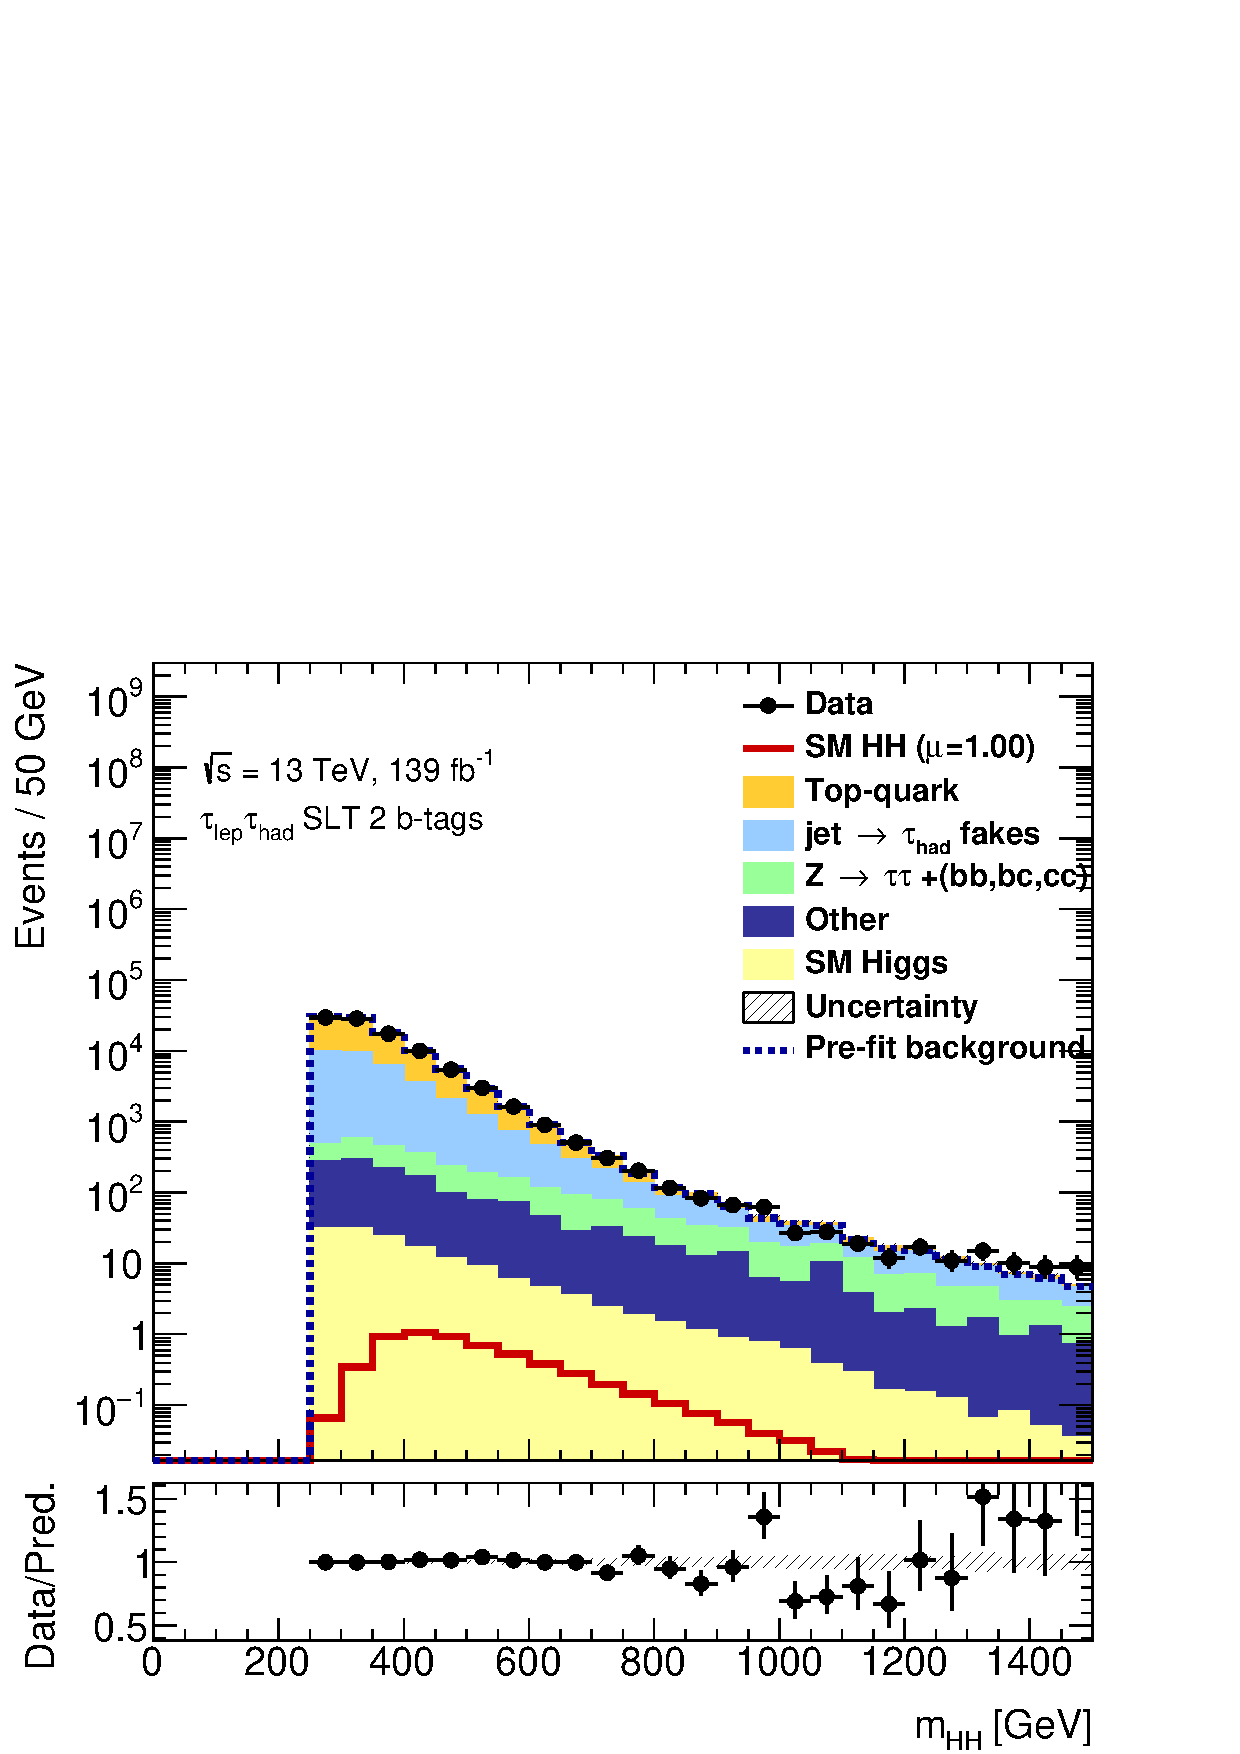
\includegraphics[width=.32\textwidth]{figures/results/HH/LepHad/Region_BMin0_incJet1_distMhh_J2_D_T2_SpcTauLH_Y2015_LTT0_L1_GlobalFit_conditionnal_mu0log.pdf}
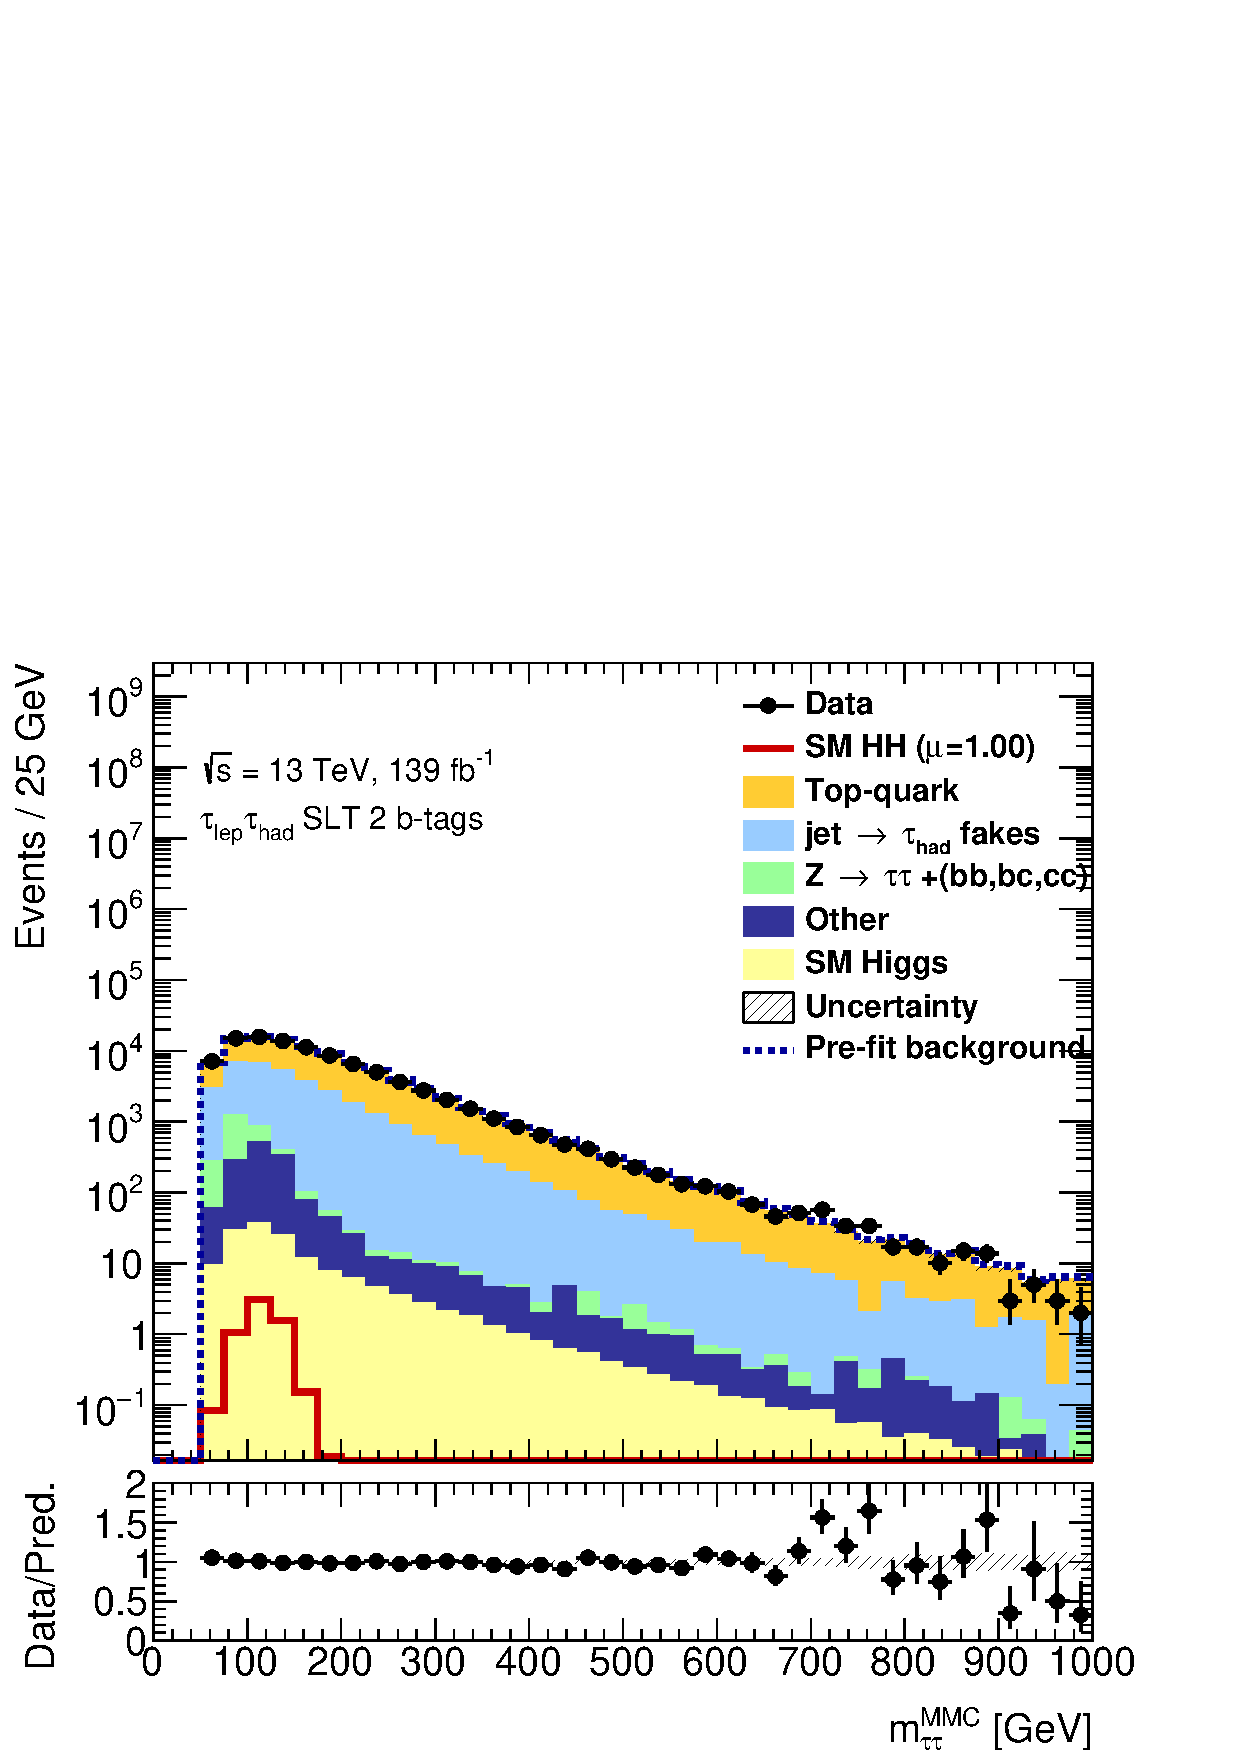
\includegraphics[width=.32\textwidth]{figures/results/HH/LepHad/Region_BMin0_incJet1_distmMMC_J2_D_T2_SpcTauLH_Y2015_LTT0_L1_GlobalFit_conditionnal_mu0log.pdf}
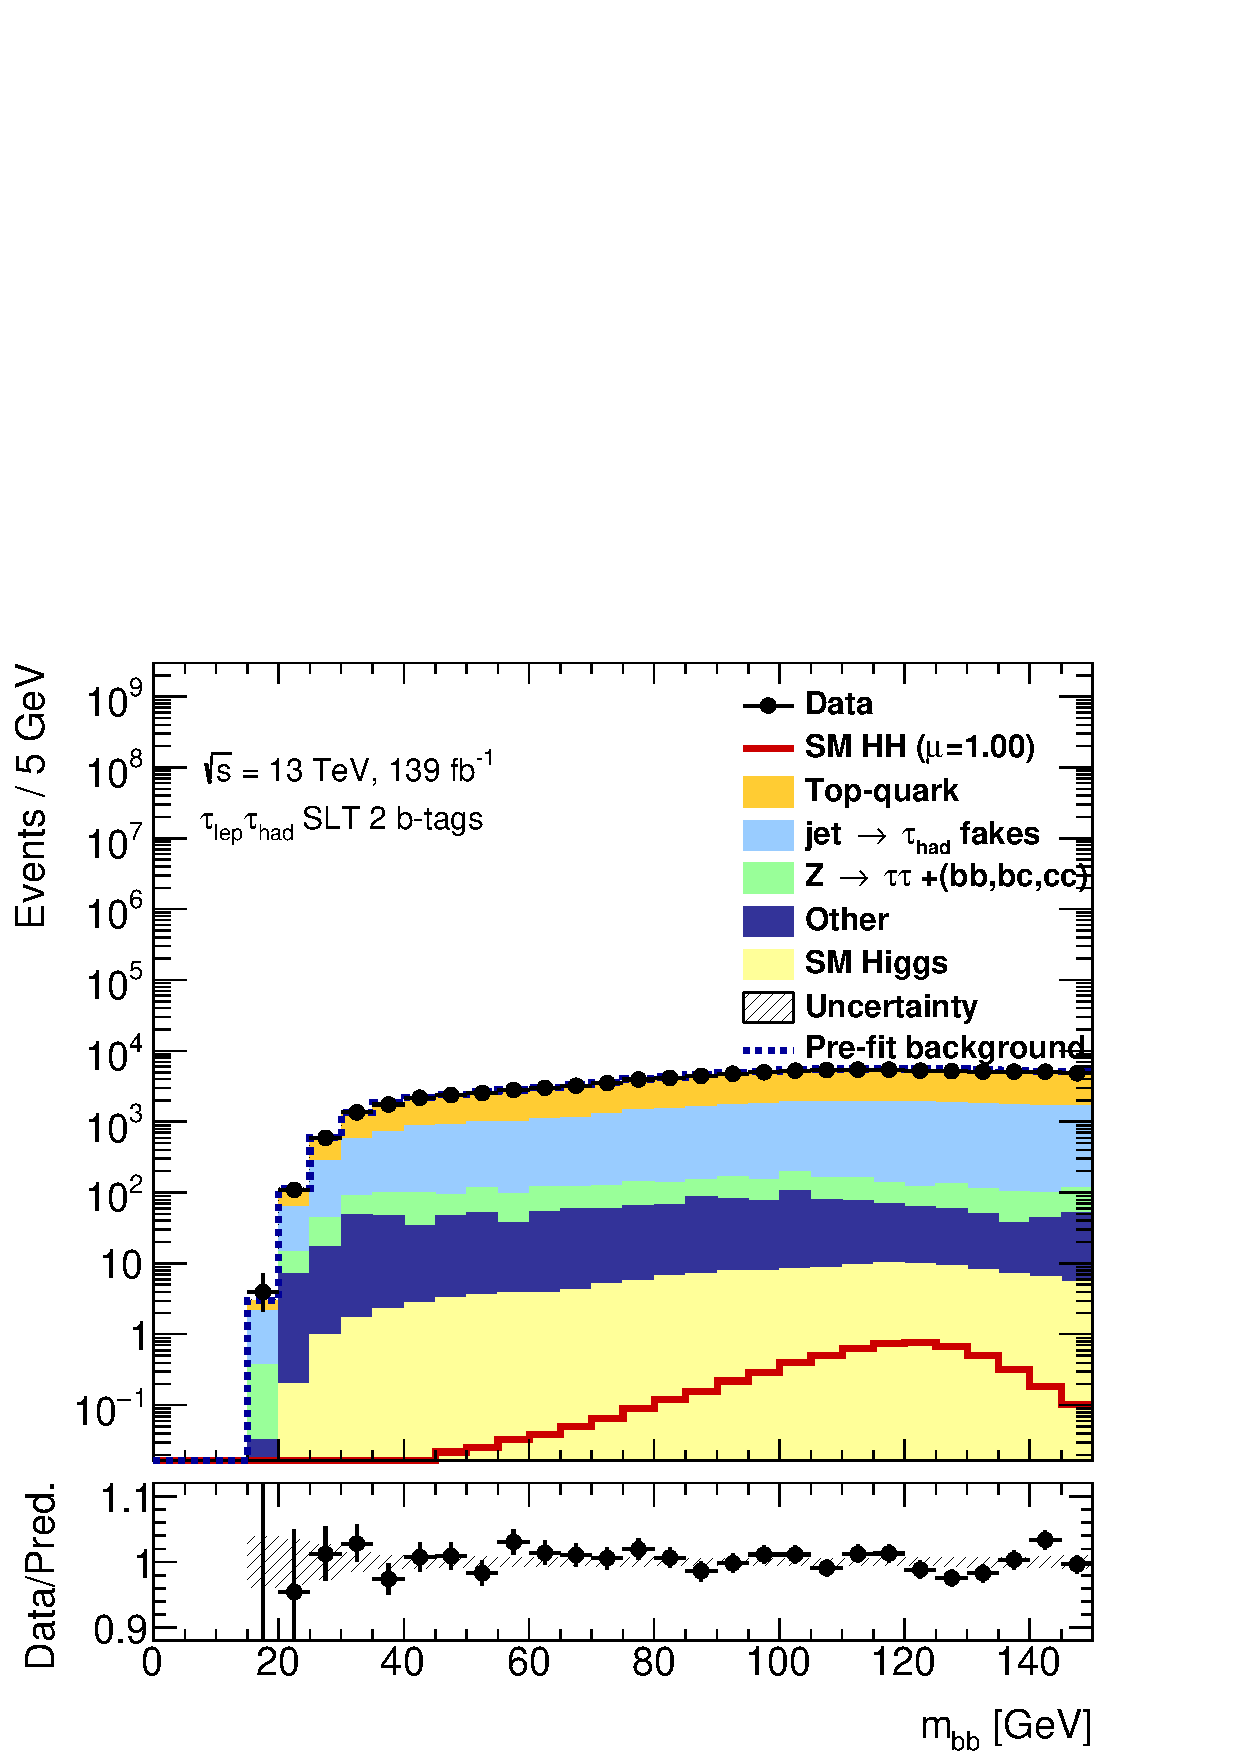
\includegraphics[width=.32\textwidth]{figures/results/HH/LepHad/Region_BMin0_incJet1_distmbb_J2_D_T2_SpcTauLH_Y2015_LTT0_L1_GlobalFit_conditionnal_mu0log.pdf} \\
\includegraphics[width=.32\textwidth]{figures/results/HH/LepHad/Region_BMin0_incJet1_distDRTauTau_J2_D_T2_SpcTauLH_Y2015_LTT0_L1_GlobalFit_conditionnal_mu0log.pdf}
\includegraphics[width=.32\textwidth]{figures/results/HH/LepHad/Region_BMin0_incJet1_distdRbb_J2_D_T2_SpcTauLH_Y2015_LTT0_L1_GlobalFit_conditionnal_mu0log.pdf}
\includegraphics[width=.32\textwidth]{figures/results/HH/LepHad/Region_BMin0_incJet1_distdPhiHBB_J2_D_T2_SpcTauLH_Y2015_LTT0_L1_GlobalFit_conditionnal_mu0log.pdf} \\
\includegraphics[width=.32\textwidth]{figures/results/HH/LepHad/Region_BMin0_incJet1_distdPtLepTau_J2_D_T2_SpcTauLH_Y2015_LTT0_L1_GlobalFit_conditionnal_mu0log.pdf}
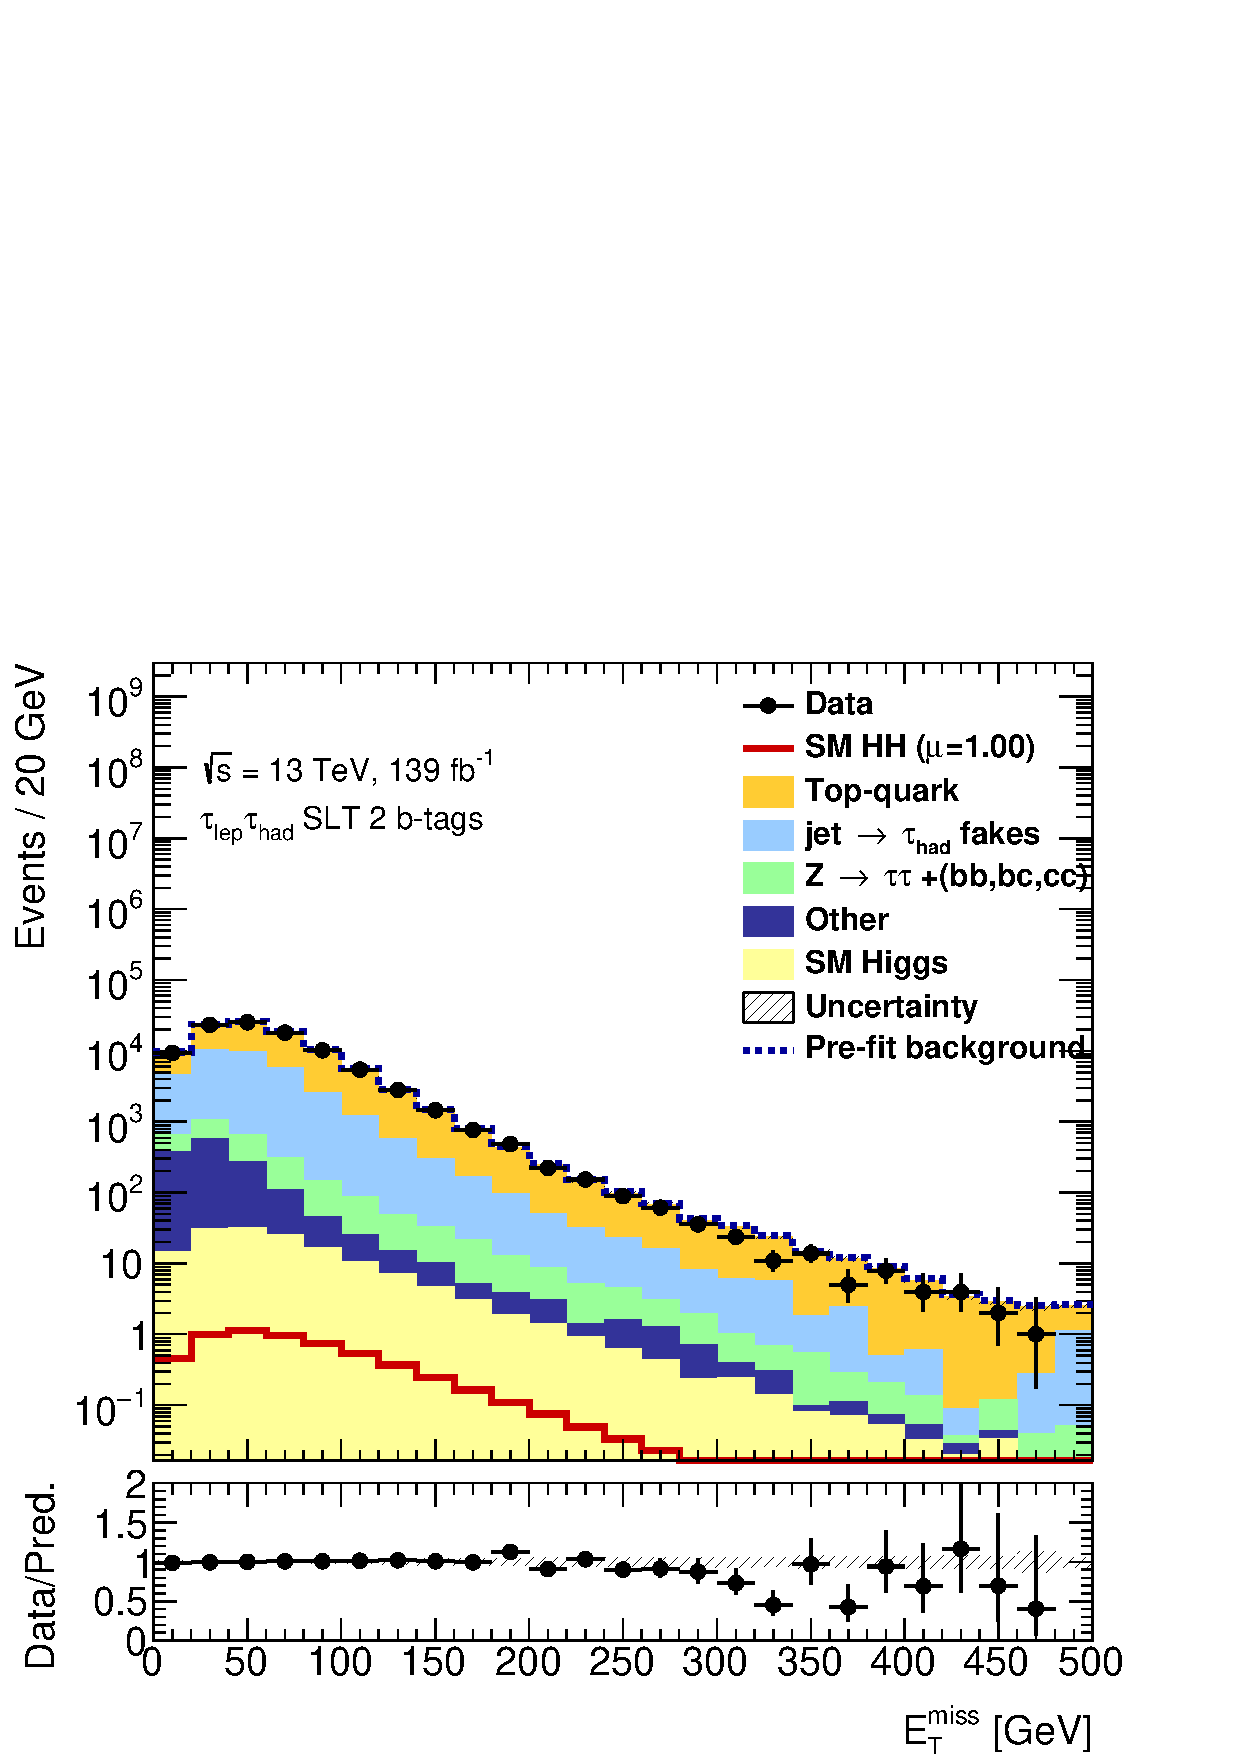
\includegraphics[width=.32\textwidth]{figures/results/HH/LepHad/Region_BMin0_incJet1_distMET_J2_D_T2_SpcTauLH_Y2015_LTT0_L1_GlobalFit_conditionnal_mu0log.pdf}
\includegraphics[width=.32\textwidth]{figures/results/HH/LepHad/Region_BMin0_incJet1_distMETCent_J2_D_T2_SpcTauLH_Y2015_LTT0_L1_GlobalFit_conditionnal_mu0log.pdf} \\
\includegraphics[width=.32\textwidth]{figures/results/HH/LepHad/Region_BMin0_incJet1_distMtW_J2_D_T2_SpcTauLH_Y2015_LTT0_L1_GlobalFit_conditionnal_mu0log.pdf}
\includegraphics[width=.32\textwidth]{figures/results/HH/LepHad/Region_BMin0_incJet1_distpTB2_J2_D_T2_SpcTauLH_Y2015_LTT0_L1_GlobalFit_conditionnal_mu0log.pdf}
\caption{Post-fit PNN/NN input variable distributions in the di-Higgs $bb\lephad$ SLT signal region.}
\label{fig:sltmvainputspostfit}
\end{figure}

\begin{figure}
\centering
\includegraphics[width=.32\textwidth]{figures/results/HH/LepHad/Region_BMin0_incJet1_distMhh_J2_D_T2_SpcTauLH_Y2015_LTT1_L1_GlobalFit_conditionnal_mu0log.pdf}
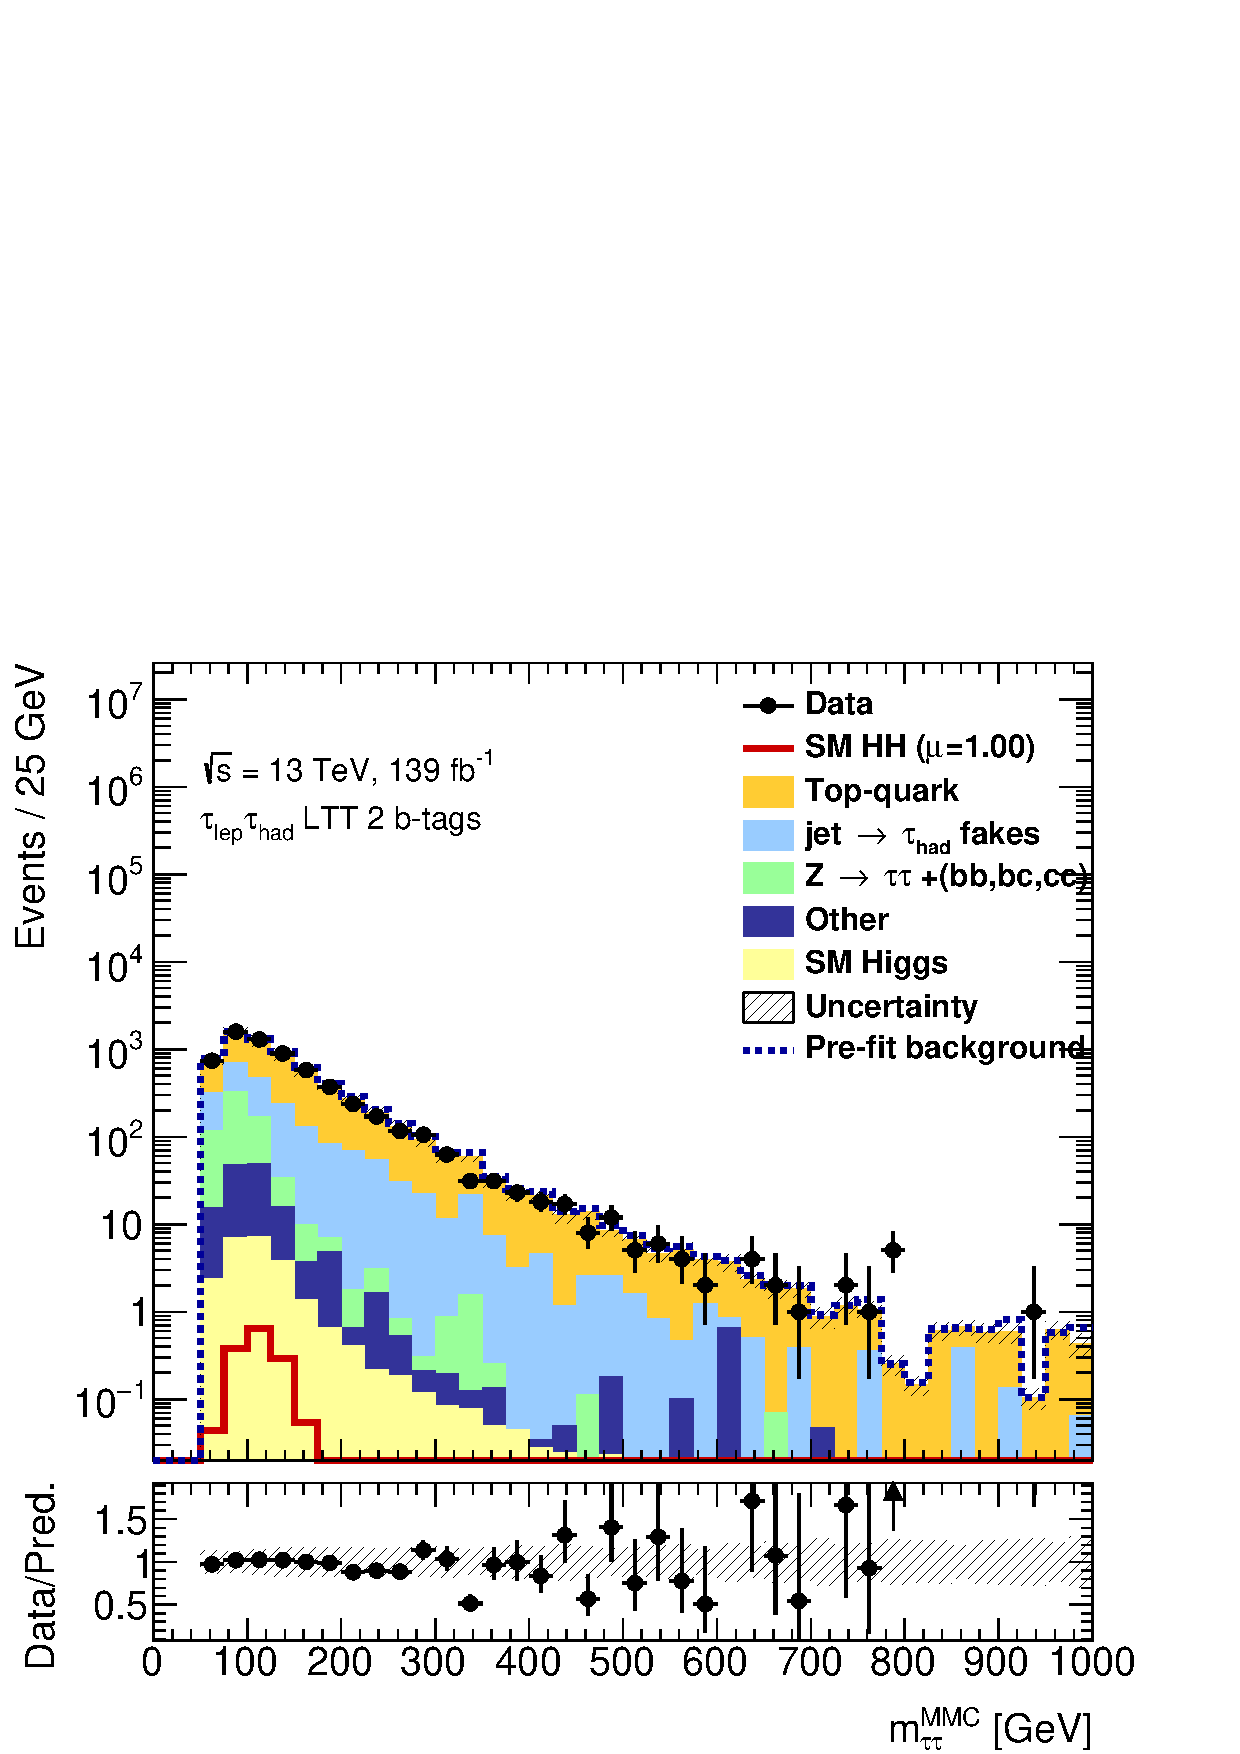
\includegraphics[width=.32\textwidth]{figures/results/HH/LepHad/Region_BMin0_incJet1_distmMMC_J2_D_T2_SpcTauLH_Y2015_LTT1_L1_GlobalFit_conditionnal_mu0log.pdf}
\includegraphics[width=.32\textwidth]{figures/results/HH/LepHad/Region_BMin0_incJet1_distmbb_J2_D_T2_SpcTauLH_Y2015_LTT1_L1_GlobalFit_conditionnal_mu0log.pdf} \\
\includegraphics[width=.32\textwidth]{figures/results/HH/LepHad/Region_BMin0_incJet1_distDRTauTau_J2_D_T2_SpcTauLH_Y2015_LTT1_L1_GlobalFit_conditionnal_mu0log.pdf}
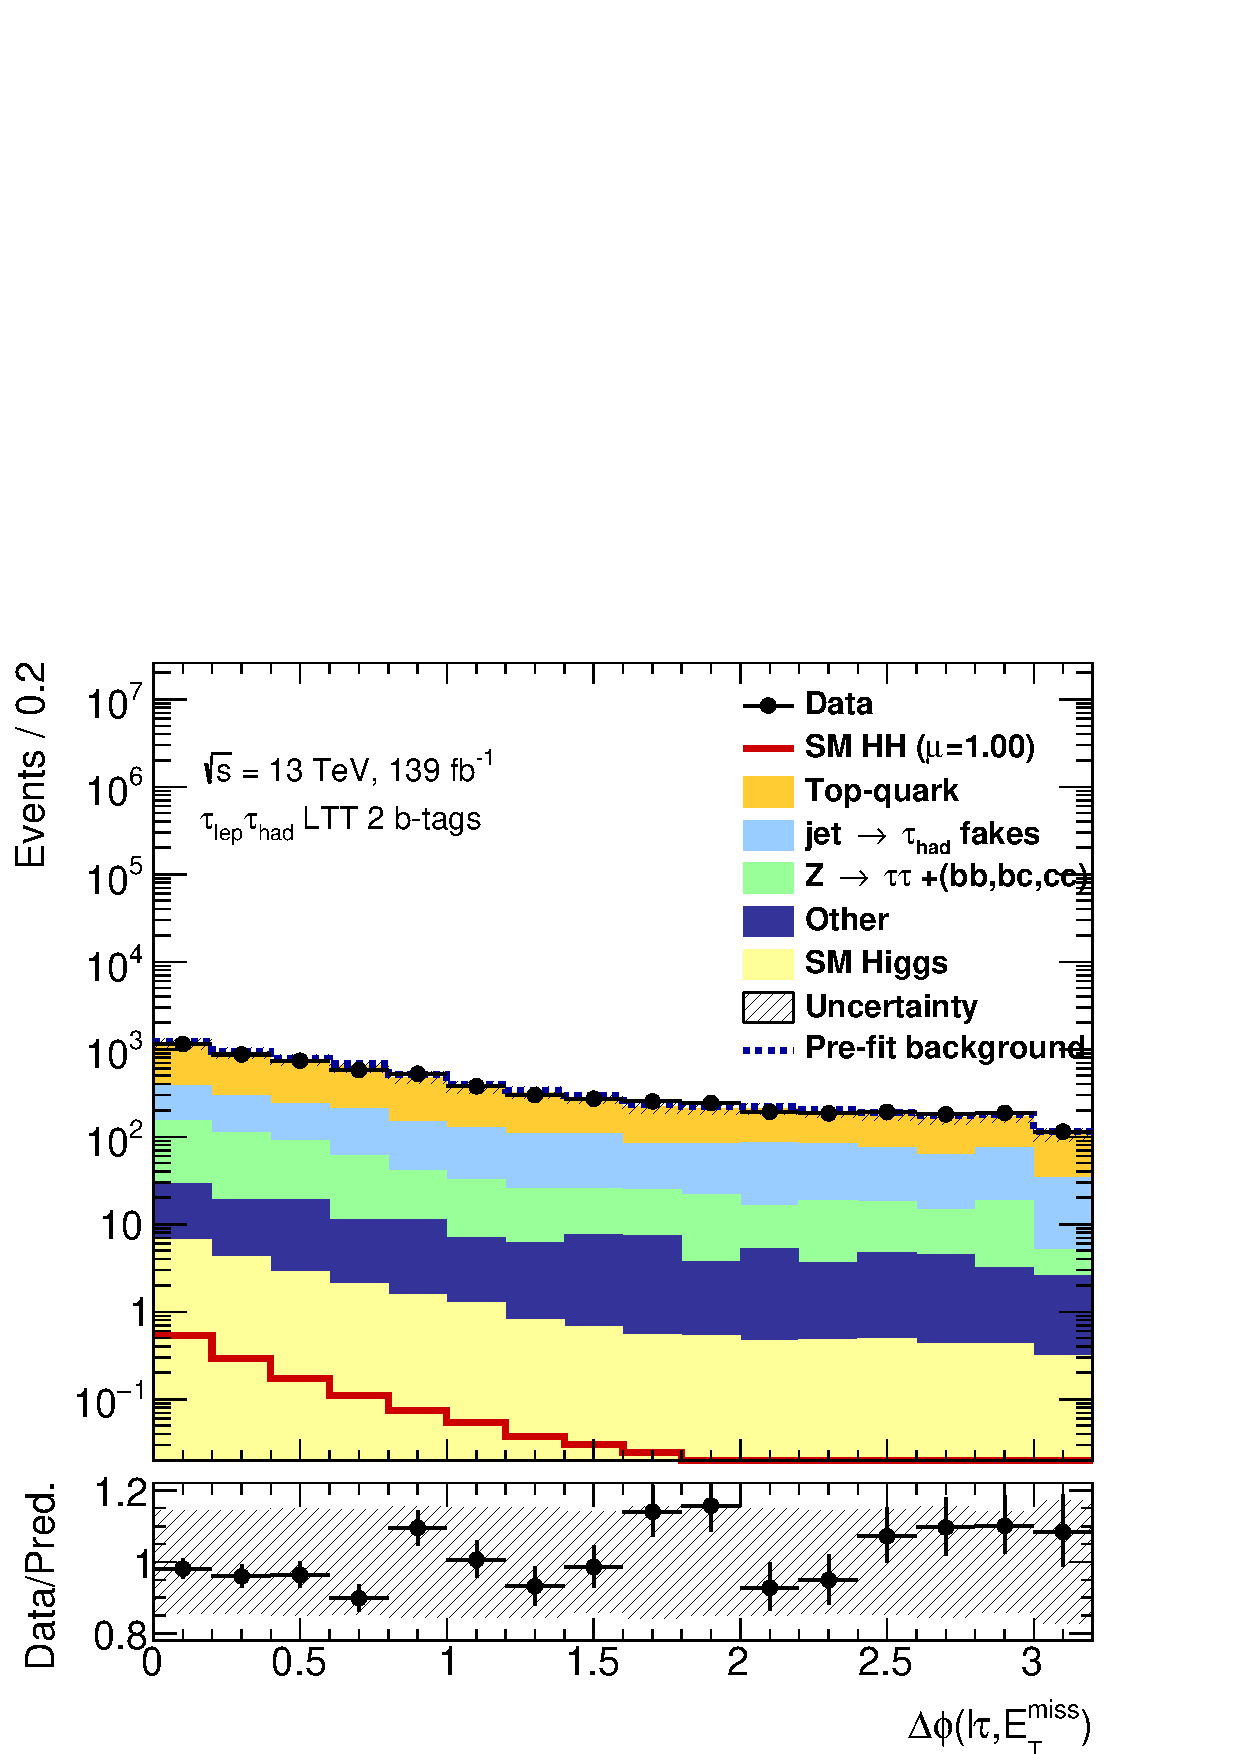
\includegraphics[width=.32\textwidth]{figures/results/HH/LepHad/Region_BMin0_incJet1_distdPhiHttMET_J2_D_T2_SpcTauLH_Y2015_LTT1_L1_GlobalFit_conditionnal_mu0log.pdf}
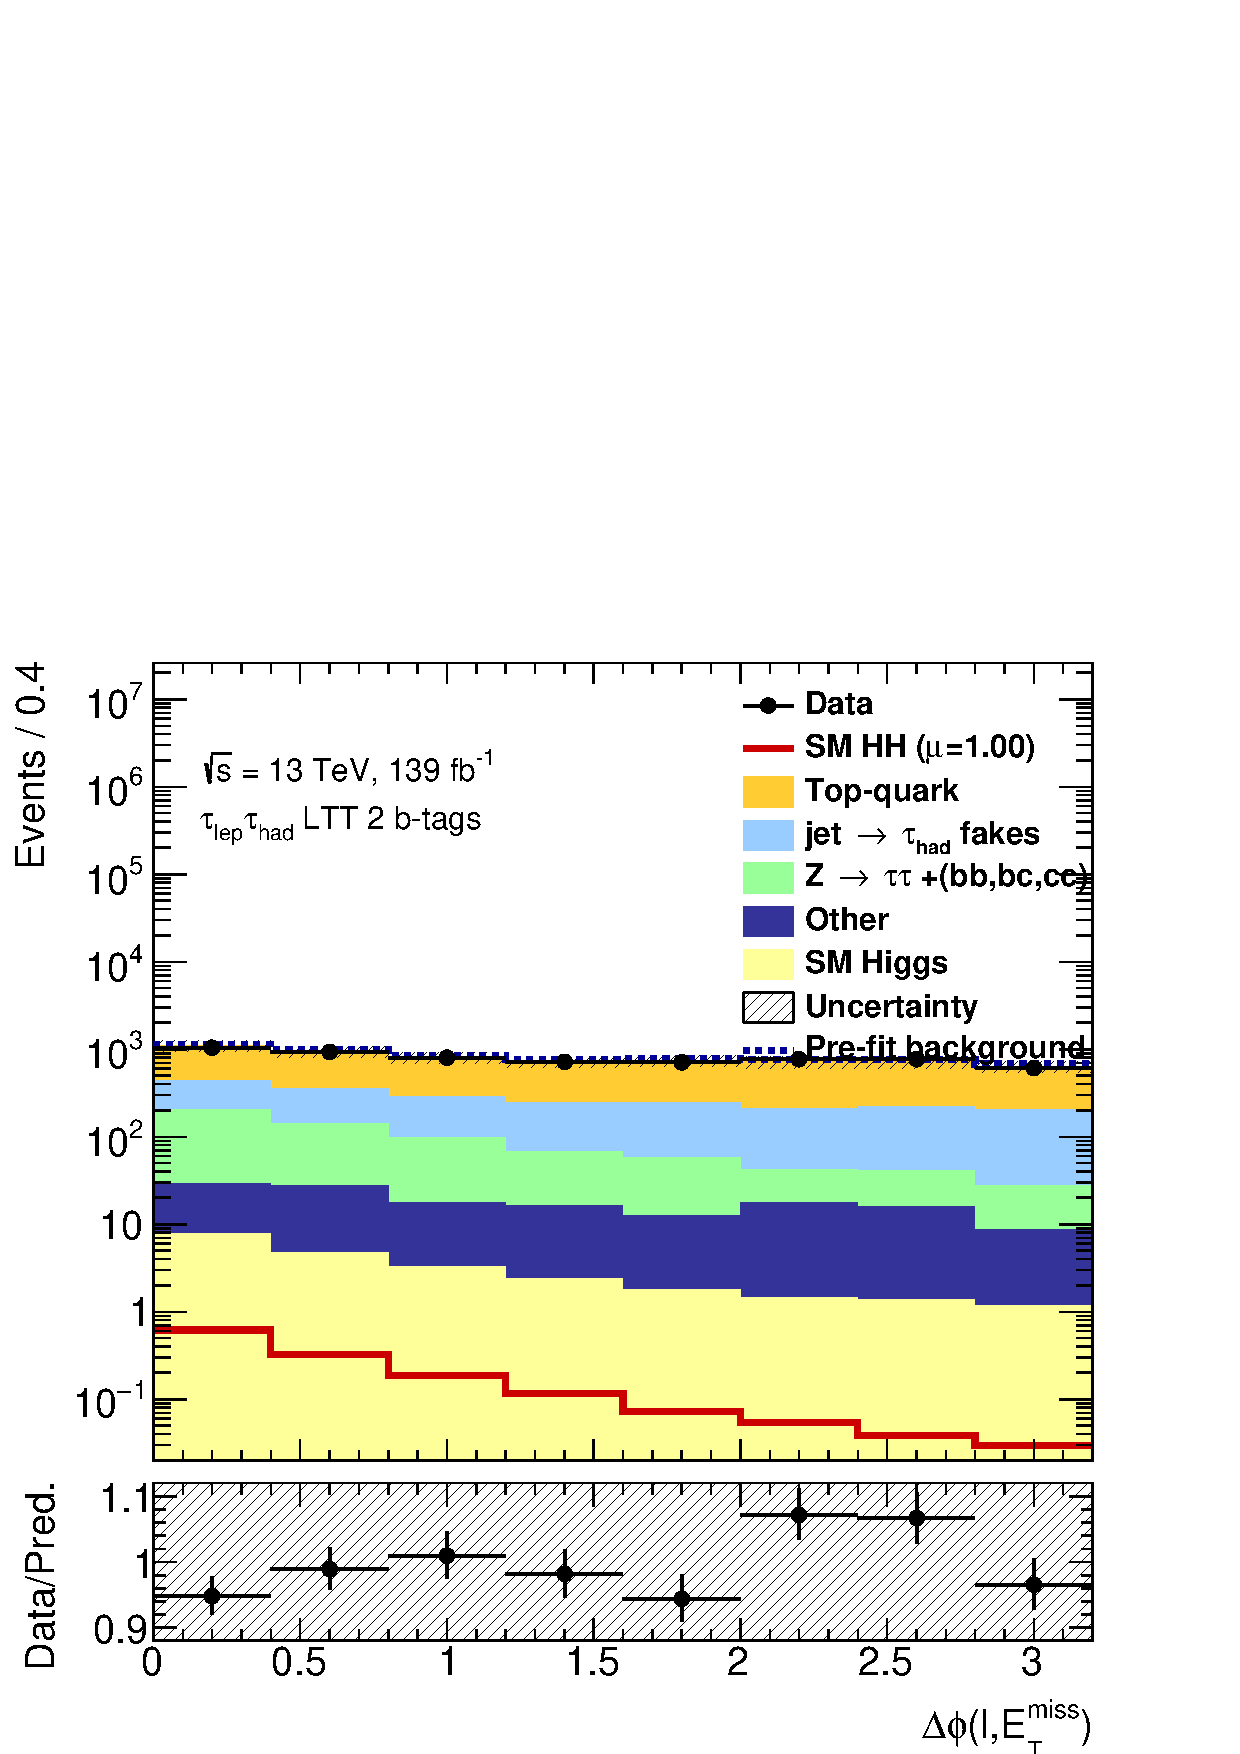
\includegraphics[width=.32\textwidth]{figures/results/HH/LepHad/Region_BMin0_incJet1_distdPhiLep0MET_J2_D_T2_SpcTauLH_Y2015_LTT1_L1_GlobalFit_conditionnal_mu0log.pdf} \\
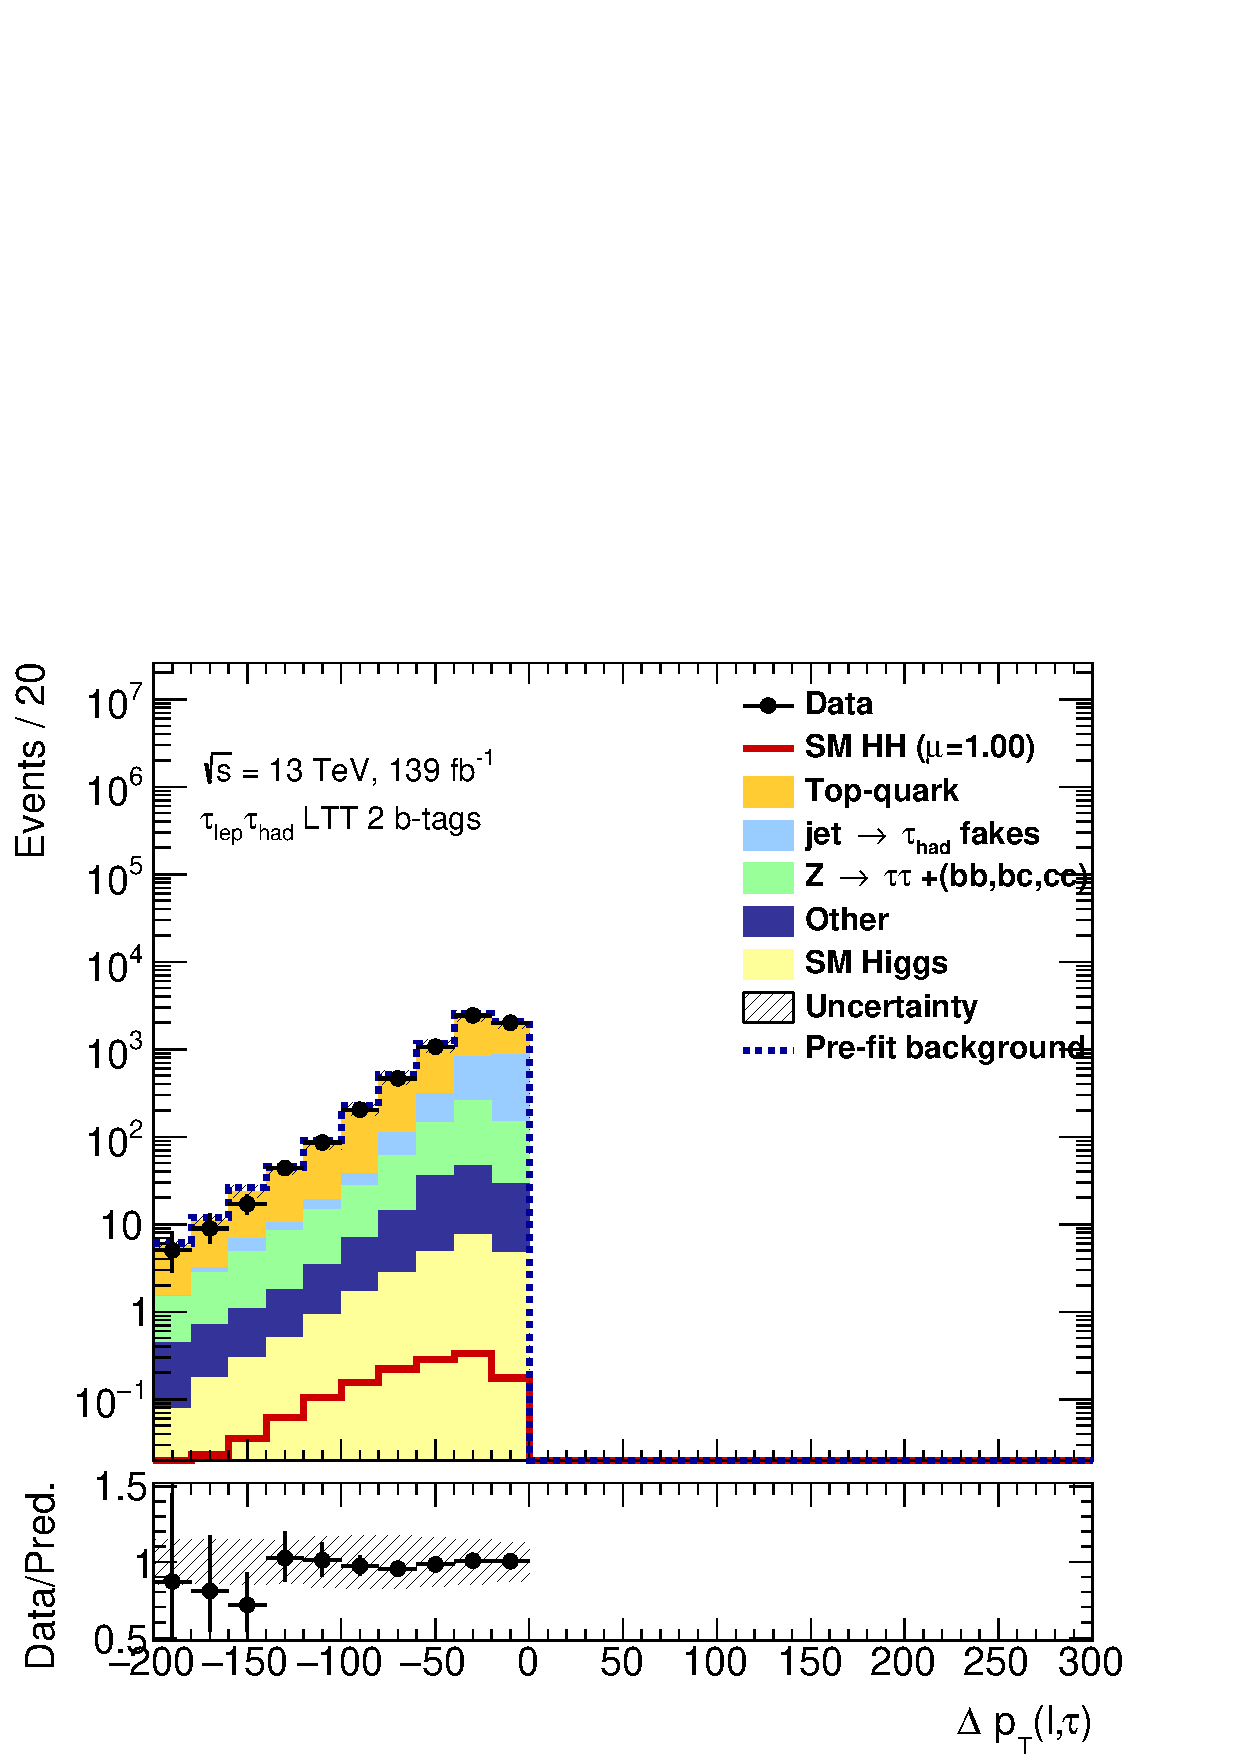
\includegraphics[width=.32\textwidth]{figures/results/HH/LepHad/Region_BMin0_incJet1_distdPtLepTau_J2_D_T2_SpcTauLH_Y2015_LTT1_L1_GlobalFit_conditionnal_mu0log.pdf}
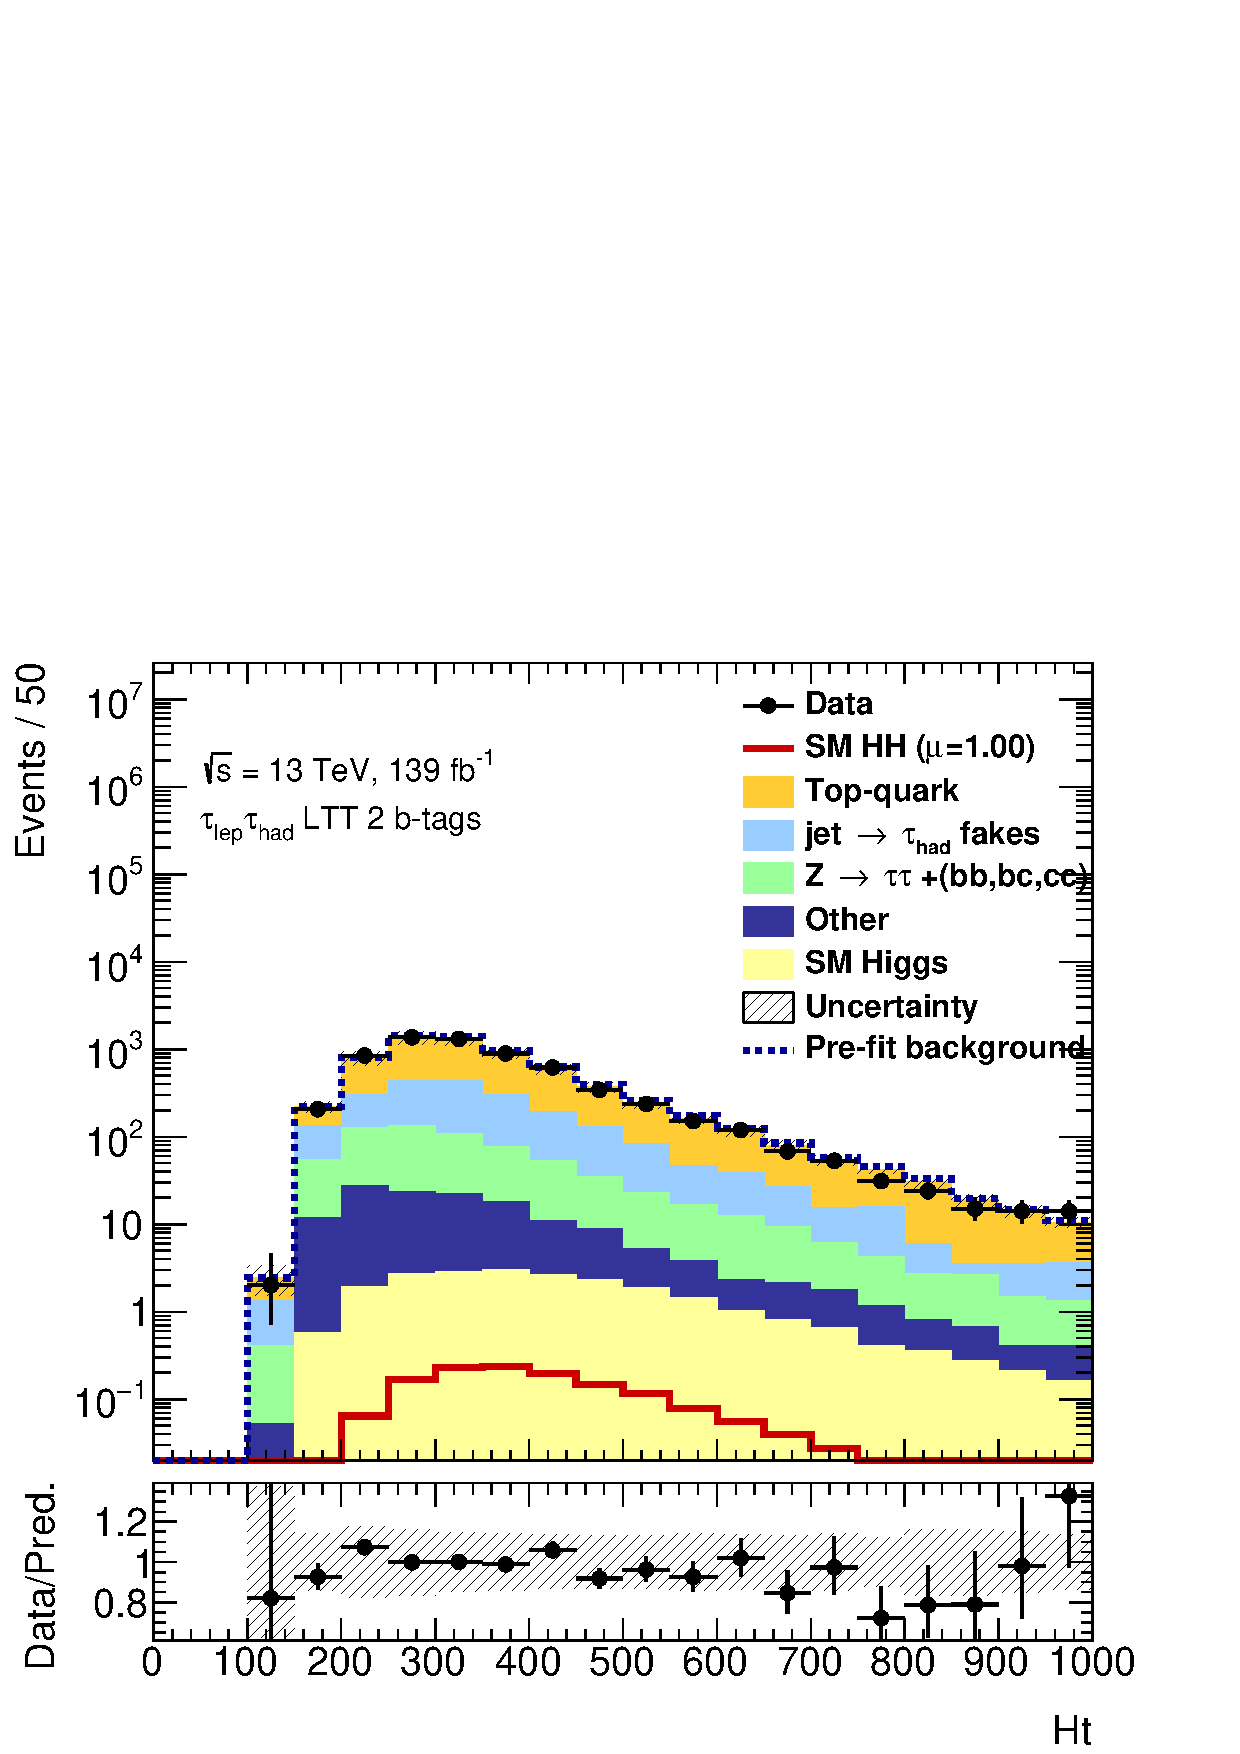
\includegraphics[width=.32\textwidth]{figures/results/HH/LepHad/Region_BMin0_incJet1_distHt_J2_D_T2_SpcTauLH_Y2015_LTT1_L1_GlobalFit_conditionnal_mu0log.pdf}
\caption{Post-fit PNN/NN input variable distributions in the di-Higgs $bb\lephad$ LTT signal region.}
\label{fig:lttmvainputspostfit}
\end{figure}


\begin{figure}
\centering
\subfloat[]
   {\includegraphics[width=.45\textwidth]{figures/results/HH/LepHad/Region_BMin0_incJet1_dist300_J2_D2HDMPNN_T2_SpcTauLH_Y2015_LTT0_L1_GlobalFit_conditionnal_mu0log.pdf}}\quad
\subfloat[]
   {\includegraphics[width=.45\textwidth]{figures/results/HH/LepHad/Region_BMin0_incJet1_dist500_J2_D2HDMPNN_T2_SpcTauLH_Y2015_LTT0_L1_GlobalFit_conditionnal_mu0log.pdf}} \quad
\subfloat[]
   {\includegraphics[width=.45\textwidth]{figures/results/HH/LepHad/Region_BMin0_incJet1_dist1000_J2_D2HDMPNN_T2_SpcTauLH_Y2015_LTT0_L1_GlobalFit_conditionnal_mu0log.pdf}}\quad
\subfloat[]
   {\includegraphics[width=.45\textwidth]{figures/results/HH/LepHad/Region_BMin0_incJet1_dist1600_J2_D2HDMPNN_T2_SpcTauLH_Y2015_LTT0_L1_GlobalFit_conditionnal_mu0log.pdf}}\quad
\subfloat[]
   {\includegraphics[width=.45\textwidth]{figures/results/HH/LepHad/Region_BMin0_incJet1_distNN_J2_DSM_T2_SpcTauLH_Y2015_LTT0_L1_GlobalFit_conditionnal_mu0log.pdf}}\quad
\caption{Post-fit PNN score distributions for the $300, 500, 1000, 1600$ GeV mass points and post-fit SM NN distribution in the di-Higgs $bb\lephad$ SLT signal region from the \lephad background-only fit. The uncertainty band includes the systematic uncertainties.}
\label{fig:LepHadSLTPostfitPNNScoreDistributions}
\end{figure}

\begin{figure}
\centering
\subfloat[]
   {\includegraphics[width=.45\textwidth]{figures/results/HH/LepHad/Region_BMin0_incJet1_dist300_J2_D2HDMPNN_T2_SpcTauLH_Y2015_LTT1_L1_GlobalFit_conditionnal_mu0log.pdf}}\quad
\subfloat[]
   {\includegraphics[width=.45\textwidth]{figures/results/HH/LepHad/Region_BMin0_incJet1_dist500_J2_D2HDMPNN_T2_SpcTauLH_Y2015_LTT1_L1_GlobalFit_conditionnal_mu0log.pdf}} \quad
\subfloat[]
   {\includegraphics[width=.45\textwidth]{figures/results/HH/LepHad/Region_BMin0_incJet1_dist1000_J2_D2HDMPNN_T2_SpcTauLH_Y2015_LTT1_L1_GlobalFit_conditionnal_mu0log.pdf}}\quad
\subfloat[]
   {\includegraphics[width=.45\textwidth]{figures/results/HH/LepHad/Region_BMin0_incJet1_dist1600_J2_D2HDMPNN_T2_SpcTauLH_Y2015_LTT1_L1_GlobalFit_conditionnal_mu0log.pdf}}\quad
\subfloat[]
   {\includegraphics[width=.45\textwidth]{figures/results/HH/LepHad/Region_BMin0_incJet1_distNN_J2_DSM_T2_SpcTauLH_Y2015_LTT1_L1_GlobalFit_conditionnal_mu0log.pdf}}\quad
\caption{Post-fit PNN score distributions for the $300, 500, 1000, 1600$ GeV mass points and post-fit SM NN distribution in the di-Higgs $bb\lephad$ LTT signal region from the \lephad background-only fit. The uncertainty band includes the systematic uncertainties.}
\label{fig:LepHadLTTPostfitPNNScoreDistributions}
\end{figure}

\begin{figure} 
\centering
\includegraphics[ angle =270]{figures/results/HH/HadHad/HadHadFit21062021/PullsAndRankings/NP_allExceptGammas_2HDM300.pdf}
\caption{NP pulls for the di-Higgs \hadhad fit for the unconditional fit to the Asimov dataset built with $\mu=0$ (red) and to data (black) for the 300 GeV resonant fit (inputs from 17\textunderscore 06\textunderscore 2021, fit from 21\textunderscore 06\textunderscore 2021).}
\label{fig:HadHadPostfitNPPulls2HDM300}
\end{figure}

\begin{figure}
\centering
\includegraphics[angle=270]{figures/results/HH/HadHad/HadHadFit21062021/PullsAndRankings/NP_allExceptGammas_2HDM500.pdf}
\caption{NP pulls for the di-Higgs \hadhad fit for the unconditional  fit to the Asimov dataset built with $\mu=0$ (red) and to data (black) for the 500 GeV  resonant fit (inputs from 17\textunderscore 06\textunderscore 2021, fit from 21\textunderscore 06\textunderscore 2021).}
\label{fig:HadHadPostfitNPPulls2HDM500}
\end{figure}

\begin{figure}
\centering
\includegraphics[angle=270]{figures/results/HH/HadHad/HadHadFit21062021/PullsAndRankings/NP_allExceptGammas_2HDM1000.pdf}
\caption{NP pulls for the di-Higgs \hadhad fit for the unconditional fit to the Asimov dataset built with $\mu=0$ (red) and to data (black) for the 1000 GeV resonant fit (inputs from 17\textunderscore 06\textunderscore 2021, fit from 21\textunderscore 06\textunderscore 2021).}
\label{fig:HadHadPostfitNPPulls2HDM1000}
\end{figure}

\begin{figure}
\centering
\includegraphics[angle=270]{figures/results/HH/HadHad/HadHadFit21062021/PullsAndRankings/NP_allExceptGammas_2HDM1600.pdf}
\caption{NP pulls for the di-Higgs \hadhad fit for the unconditional fit to the Asimov dataset built with $\mu=0$ (red) and to data (black) for the 1600 GeV resonant fit (inputs from 17\textunderscore 06\textunderscore 2021, fit from 21\textunderscore 06\textunderscore 2021).}
\label{fig:HadHadPostfitNPPulls2HDM1600}
\end{figure}

\begin{figure}
\centering
\includegraphics[width=.9\textwidth]{figures/results/HH/HadHad/HadHadFit14072021/PullsAndRankings/NP_allExceptGammas_SM.pdf}
\caption{NP pulls for the di-Higgs \hadhad fit for the unconditional  fit to the Asimov dataset built with $\mu=0$ (red) and to data (black) for the SM fit (inputs from 17\textunderscore 06\textunderscore 2021, fit from 14\textunderscore 07\textunderscore 2021).}
\label{fig:HadHadPostfitNPPullsSM}
\end{figure}

\begin{figure}
\centering
\includegraphics[angle=270]{figures/results/HH/LepHad/NP_allExceptGammas_2HDM300_SLT.pdf}
\caption{NP pulls for the di-Higgs \lephad SLT fit for the fit to the Asimov dataset built with $\mu=0$ (red) and for the fit to data (black) for the 300 GeV resonant fit.}
\label{fig:LepHadPostfitNPPulls2HDM300SLT}
\end{figure}

\begin{figure}
\centering
\includegraphics[angle=270]{figures/results/HH/LepHad/NP_allExceptGammas_2HDM500_SLT.pdf}
\caption{NP pulls for the di-Higgs \lephad SLT fit for the fit to the Asimov dataset built with $\mu=0$ (red) and for the fit to data (black) for the 500 GeV  resonant fit.}
\label{fig:LepHadPostfitNPPulls2HDM500SLT}
\end{figure}

\begin{figure}
\centering
\includegraphics[angle=270]{figures/results/HH/LepHad/NP_allExceptGammas_2HDM1000_SLT.pdf}
\caption{NP pulls for the di-Higgs \lephad SLT fit for the fit to the Asimov dataset built with $\mu=0$ (red) and for the fit to data (black) for the 1000 GeV resonant fit.}
\label{fig:LepHadPostfitNPPulls2HDM1000SLT}
\end{figure}

\begin{figure}
\centering
\includegraphics[angle=270]{figures/results/HH/LepHad/NP_allExceptGammas_2HDM1600_SLT.pdf}
\caption{NP pulls for the di-Higgs \lephad SLT fit for the fit to the Asimov dataset built with $\mu=0$ (red) and for the fit to data (black) for the 1600 GeV resonant fit.}
\label{fig:LepHadPostfitNPPulls2HDM1600SLT}
\end{figure}

\begin{figure}
\centering
\includegraphics[angle=270]{figures/results/HH/LepHad/NP_allExceptGammas_SM_SLT.pdf}
\caption{NP pulls for the di-Higgs \lephad SLT fit for the fit to the Asimov dataset built with $\mu=0$ (red) and for the fit to data (black) for the SM fit.}
\label{fig:LepHadPostfitNPPullsSMSLT}
\end{figure}

\begin{figure}
\centering
\includegraphics[angle=270]{figures/results/HH/LepHad/NP_allExceptGammas_2HDM300_LTT.pdf}
\caption{NP pulls for the di-Higgs \lephad LTT fit for the fit to the Asimov dataset built with $\mu=0$ (red) and for the fit to data (black) for the 300 GeV resonant fit.}
\label{fig:LepHadPostfitNPPulls2HDM300LTT}
\end{figure}

\begin{figure}
\centering
\includegraphics[angle=270]{figures/results/HH/LepHad/NP_allExceptGammas_2HDM500_LTT.pdf}
\caption{NP pulls for the di-Higgs \lephad LTT fit for the fit to the Asimov dataset built with $\mu=0$ (red) and for the fit to data (black) for the 500 GeV resonant fit.}
\label{fig:LepHadPostfitNPPulls2HDM500LTT}
\end{figure}

\begin{figure}
\centering
\includegraphics[angle=270]{figures/results/HH/LepHad/NP_allExceptGammas_2HDM1000_LTT.pdf}
\caption{NP pulls for the di-Higgs \lephad LTT fit for the fit to the Asimov dataset built with $\mu=0$ (red) and for the fit to data (black) for the 1000 GeV resonant fit.}
\label{fig:LepHadPostfitNPPulls2HDM1000LTT}
\end{figure}

\begin{figure}
\centering
\includegraphics[angle=270]{figures/results/HH/LepHad/NP_allExceptGammas_2HDM1600_LTT.pdf}
\caption{NP pulls for the di-Higgs \lephad LTT fit for the fit to the Asimov dataset built with $\mu=0$ (red) and for the fit to data (black) for the 1600 GeV resonant fit.}
\label{fig:LepHadPostfitNPPulls2HDM1600LTT}
\end{figure}

\begin{figure}
\centering
\includegraphics[angle=270]{figures/results/HH/LepHad/NP_allExceptGammas_SM_LTT.pdf}
\caption{NP pulls for the di-Higgs \lephad LTT fit for the fit to the Asimov dataset built with $\mu=0$ (red) and for the fit to data (black) for the SM fit.}
\label{fig:LepHadPostfitNPPullsSMLTT}
\end{figure}

\begin{figure}
\centering
\includegraphics[angle=270]{figures/results/HH/LepHad/NP_allExceptGammas_2HDM300.pdf}
\caption{NP pulls for the di-Higgs \lephad fit for the fit to the Asimov dataset built with $\mu=0$ (red) and for the fit to data (black) for the 300 GeV resonant fit.}
\label{fig:LepHadPostfitNPPulls2HDM300}
\end{figure}

\begin{figure}
\centering
\includegraphics[angle=270]{figures/results/HH/LepHad/NP_allExceptGammas_2HDM500.pdf}
\caption{NP pulls for the di-Higgs \lephad fit for the fit to the Asimov dataset built with $\mu=0$ (red) and for the fit to data (black) for the 500 GeV  resonant fit.}
\label{fig:LepHadPostfitNPPulls2HDM500}
\end{figure}

\begin{figure}
\centering
\includegraphics[angle=270]{figures/results/HH/LepHad/NP_allExceptGammas_2HDM1000.pdf}
\caption{NP pulls for the di-Higgs \lephad fit for the fit to the Asimov dataset built with $\mu=0$ (red) and for the fit to data (black) for the 1000 GeV resonant fit.}
\label{fig:LepHadPostfitNPPulls2HDM1000}
\end{figure}

\begin{figure}
\centering
\includegraphics[angle=270]{figures/results/HH/LepHad/NP_allExceptGammas_2HDM1600.pdf}
\caption{NP pulls for the di-Higgs \lephad fit for the fit to the Asimov dataset built with $\mu=0$ (red) and for the fit to data (black) for the 1600 GeV resonant fit.}
\label{fig:LepHadPostfitNPPulls2HDM1600}
\end{figure}

\begin{figure}
\centering
\includegraphics[angle=270]{figures/results/HH/LepHad/NP_allExceptGammas_SM.pdf}
\caption{NP pulls for the di-Higgs \lephad fit for the fit to the Asimov dataset built with $\mu=0$ (red) and for the fit to data (black) for the SM fit.}
\label{fig:LepHadPostfitNPPullsSM}
\end{figure}

\clearpage

\begin{figure}
\centering
\subfloat[]
   {\includegraphics[width=.45\textwidth]{figures/results/HH/LepHad/NP_Top_300.pdf}}\qquad
\subfloat[]
   {\includegraphics[width=.45\textwidth]{figures/results/HH/LepHad/NP_Top_500.pdf}}\qquad
\subfloat[]
   {\includegraphics[width=.45\textwidth]{figures/results/HH/LepHad/NP_Top_1000.pdf}}\qquad
\subfloat[]
   {\includegraphics[width=.45\textwidth]{figures/results/HH/LepHad/NP_Top_1600.pdf}}\qquad
\subfloat[]
   {\includegraphics[width=.45\textwidth]{figures/results/HH/LepHad/NP_Top_SM.pdf}}\qquad
\caption{ttbar modeling related NP pulls for the $300, 500, 1000, 1600$ GeV mass points and SM case in the di-Higgs \lephad fit to data.} 
\label{fig:LepHadPostfitNPPullsTop}
\end{figure}

\begin{figure}
\centering
\includegraphics[width=.8\textwidth]{figures/results/HH/HadHad/HadHadFit21062021/PullsAndRankings/pulls_SigXsecOverSM_300.pdf}
\caption{NP rankings for the di-Higgs \hadhad fit to data for the 300 GeV resonant fit (inputs from 17\textunderscore 06\textunderscore 2021, fit from 21\textunderscore 06\textunderscore 2021).}
\label{fig:HadHadPostfitNPRankings2HDM300}
\end{figure}

\begin{figure}
\centering
\includegraphics[width=.8\textwidth]{figures/results/HH/HadHad/HadHadFit21062021/PullsAndRankings/pulls_SigXsecOverSM_500.pdf}
\caption{NP rankings for the di-Higgs \hadhad fit to data for the 500 GeV resonant fit (inputs from 17\textunderscore 06\textunderscore 2021, fit from 21\textunderscore 06\textunderscore 2021).}
\label{fig:HadHadPostfitNPRankings2HDM500}
\end{figure}

\begin{figure}
\centering
\includegraphics[width=.8\textwidth]{figures/results/HH/HadHad/HadHadFit21062021/PullsAndRankings/pulls_SigXsecOverSM_1000.pdf}
\caption{NP rankings for the di-Higgs \hadhad fit to data for the 1000 GeV resonant fit (inputs from 17\textunderscore 06\textunderscore 2021, fit from 21\textunderscore 06\textunderscore 2021).}
\label{fig:HadHadPostfitNPRankings2HDM1000}
\end{figure}

\begin{figure}
\centering
\includegraphics[width=.8\textwidth]{figures/results/HH/HadHad/HadHadFit21062021/PullsAndRankings/pulls_SigXsecOverSM_1600.pdf}
\caption{NP rankings for the di-Higgs \hadhad fit to data for the 1600 GeV resonant fit (inputs from 17\textunderscore 06\textunderscore 2021, fit from 21\textunderscore 06\textunderscore 2021).}
\label{fig:HadHadPostfitNPRankings2HDM1600}
\end{figure}

\begin{figure}
\centering
\includegraphics[width=.8\textwidth]{figures/results/HH/HadHad/HadHadFit14072021/PullsAndRankings/pulls_SigXsecOverSM_0.pdf}
\caption{NP rankings for the di-Higgs \hadhad fit to data for the SM fit (inputs from 17\textunderscore 06\textunderscore 2021, fit from 14\textunderscore 07\textunderscore 2021).}
\label{fig:HadHadPostfitNPRankingsSM}
\end{figure}

\begin{table}
\centering
\begin{tabular}{|c|c|}
\hline
Set of nuisance parameters & Fractional impact on error\\
\hline
Data statistics & $\pm 0.61$\\
Full systematics & $\pm 0.38$\\
Jet and MET & $\pm 0.05$ \\
b-tagging & $\pm 0.02$\\
Electron and Muon & $\pm 0.00$\\
Tau & $0.01$\\
Pileup reweighting & $\pm 0.00$\\
Luminosity & $\pm 0.00$\\
Fake estimation & $\pm 0.03$\\
Top modelling & $\pm 0.03$\\ 
Z+HF modelling & $\pm 0.02$\\
Single Higgs modelling & $\pm 0.00$\\
Signal modelling & $\pm 0.05$\\
Other backgrounds & $\pm 0.00$\\
MC statistics & $\pm 0.13$\\
\hline
\end{tabular}
\caption{Impact of the uncertainties on the total uncertainty on $\mu$ for the resonant 300 GeV fit in the \hadhad channel for an Asimov dataset built with $\mu$ at the expected limit. The impact is expressed as fractional impact on the signal strength parameter,  calculated by considering the square of the uncertainty on the signal strength parameter arising from a given group of uncertainties divided by the square of the total uncertainty on the signal strength parameter.  (inputs from 17\textunderscore 06\textunderscore 2021, fit from 21\textunderscore 06\textunderscore 2021)}
\label{sec:fit:tab:HadHadBreakdown2HDM300Asimov}
\end{table}

\begin{table}
\centering
\begin{tabular}{|c|c|}
\hline
Set of nuisance parameters & Fractional impact on error\\
\hline
Data statistics & $\pm 0.83$\\
Full systematics & $\pm 0.17$\\
Jet and MET & $\pm 0.01$ \\
b-tagging & $\pm 0.00$\\
Electron and Muon & $\pm 0.00$\\
Tau & $0.01$\\
Pileup reweighting & $\pm 0.00$\\
Luminosity & $\pm 0.00$\\
Fake estimation & $\pm 0.00$\\
Top modelling & $\pm 0.01$\\ 
Z+HF modelling & $\pm 0.02$\\
Single Higgs modelling & $\pm 0.01$\\
Signal modelling & $\pm 0.05$\\
Other backgrounds & $\pm 0.00$\\
MC statistics & $\pm 0.05$\\
\hline
\end{tabular}
\caption{Impact of the uncertainties on the total uncertainty on $\mu$ for the resonant 500 GeV fit in the \hadhad channel for an Asimov dataset built with $\mu$ at the expected limit. The impact is expressed as fractional impact on the signal strength parameter,  calculated by considering the square of the uncertainty on the signal strength parameter arising from a given group of uncertainties divided by the square of the total uncertainty on the signal strength parameter.  (inputs from 17\textunderscore 06\textunderscore 2021, fit from 21\textunderscore 06\textunderscore 2021)}
\label{sec:fit:tab:HadHadBreakdown2HDM500Asimov}
\end{table}

\begin{table}
\centering
\begin{tabular}{|c|c|}
\hline
Set of nuisance parameters & Fractional impact on error\\
\hline
Data statistics & $\pm 0.85$\\
Full systematics & $\pm 0.15$\\
Jet and MET & $\pm 0.00$ \\
b-tagging & $\pm 0.00$\\
Electron and Muon & $\pm 0.00$\\
Tau & $0.01$\\
Pileup reweighting & $\pm 0.00$\\
Luminosity & $\pm 0.00$\\
Fake estimation & $\pm 0.00$\\
Top modelling & $\pm 0.00$\\ 
Z+HF modelling & $\pm 0.02$\\
Single Higgs modelling & $\pm 0.02$\\
Signal modelling & $\pm 0.05$\\
Other backgrounds & $\pm 0.00$\\
MC statistics & $\pm 0.03$\\
\hline
\end{tabular}
\caption{Impact of the uncertainties on the total uncertainty on $\mu$ for the resonant 1000 GeV fit in the \hadhad channel for an Asimov dataset built with $\mu$ at the expected limit. The impact is expressed as fractional impact on the signal strength parameter,  calculated by considering the square of the uncertainty on the signal strength parameter arising from a given group of uncertainties divided by the square of the total uncertainty on the signal strength parameter.  (inputs from 17\textunderscore 06\textunderscore 2021, fit from 21\textunderscore 06\textunderscore 2021)}
\label{sec:fit:tab:HadHadBreakdown2HDM1000Asimov}
\end{table}



\begin{table}
\centering
\begin{tabular}{|c|c|}
\hline
Set of nuisance parameters & Fractional impact on error\\
\hline
Data statistics & $\pm 0.78$\\
Full systematics & $\pm 0.22$\\
Jet and MET & $\pm 0.01$ \\
b-tagging & $\pm 0.00$\\
Electron and Muon & $\pm 0.00$\\
Tau & $0.02$\\
Pileup reweighting & $\pm 0.00$\\
Luminosity & $\pm 0.00$\\
Fake estimation & $\pm 0.01$\\
Top modelling & $\pm 0.01$\\ 
Z+HF modelling & $\pm 0.01$\\
Single Higgs modelling & $\pm 0.06$\\
Signal modelling & $\pm 0.02$\\
Other backgrounds & $\pm 0.00$\\
MC statistics & $\pm 0.05$\\
\hline
\end{tabular}
\caption{Impact of the uncertainties on the total uncertainty on $\mu$ for the non-resonant SM fit in the \hadhad channel for an Asimov dataset built with $\mu$ at the expected limit. The impact is expressed as fractional impact on the signal strength parameter,  calculated by considering the square of the uncertainty on the signal strength parameter arising from a given group of uncertainties divided by the square of the total uncertainty on the signal strength parameter.  (inputs from 17\textunderscore 06\textunderscore 2021, fit from 21\textunderscore 06\textunderscore 2021)}
\label{sec:fit:tab:HadHadBreakdownSMAsimov}
\end{table}

\begin{table}
\centering
\begin{tabular}{|c|c|}
\hline
Set of nuisance parameters & Fractional impact on error\\
\hline
Data statistics & $\pm 0.65$\\
Full systematics & $\pm 0.35$\\
Jet and MET & $\pm 0.04$ \\
b-tagging & $\pm 0.00$\\
Electron and Muon & $\pm 0.00$\\
Tau & $0.01$\\
Pileup reweighting & $\pm 0.00$\\
Luminosity & $\pm 0.00$\\
Fake estimation & $\pm 0.03$\\
Top modelling & $\pm 0.03$\\ 
Z+HF modelling & $\pm 0.02$\\
Single Higgs modelling & $\pm 0.00$\\
Signal modelling & $\pm 0.02$\\
Other backgrounds & $\pm 0.00$\\
MC statistics & $\pm 0.15$\\
\hline
\end{tabular}
\caption{Impact of the uncertainties on the total uncertainty on $\mu$ for the resonant 300 GeV fit in the \hadhad channel for the observed dataset. The impact is expressed as fractional impact on the signal strength parameter,  calculated by considering the square of the uncertainty on the signal strength parameter arising from a given group of uncertainties divided by the square of the total uncertainty on the signal strength parameter.  (inputs from 17\textunderscore 06\textunderscore 2021, fit from 21\textunderscore 06\textunderscore 2021)}
\label{sec:fit:tab:HadHadBreakdown2HDM300Observed}
\end{table}

\begin{table}
\centering
\begin{tabular}{|c|c|}
\hline
Set of nuisance parameters & Fractional impact on error\\
\hline
Data statistics & $\pm 0.81$\\
Full systematics & $\pm 0.18$\\
Jet and MET & $\pm 0.01$ \\
b-tagging & $\pm 0.00$\\
Electron and Muon & $\pm 0.00$\\
Tau & $0.00$\\
Pileup reweighting & $\pm 0.00$\\
Luminosity & $\pm 0.00$\\
Fake estimation & $\pm 0.00$\\
Top modelling & $\pm 0.01$\\ 
Z+HF modelling & $\pm 0.01$\\
Single Higgs modelling & $\pm 0.02$\\
Signal modelling & $\pm 0.02$\\
Other backgrounds & $\pm 0.00$\\
MC statistics & $\pm 0.11$\\
\hline
\end{tabular}
\caption{Impact of the uncertainties on the total uncertainty on $\mu$ for the resonant 500 GeV fit in the \hadhad channel for the observed dataset. The impact is expressed as fractional impact on the signal strength parameter,  calculated by considering the square of the uncertainty on the signal strength parameter arising from a given group of uncertainties divided by the square of the total uncertainty on the signal strength parameter.  (inputs from 17\textunderscore 06\textunderscore 2021, fit from 21\textunderscore 06\textunderscore 2021)}
\label{sec:fit:tab:HadHadBreakdown2HDM500Observed}
\end{table}

\begin{table}
\centering
\begin{tabular}{|c|c|}
\hline
Set of nuisance parameters & Fractional impact on error\\
\hline
Data statistics & $\pm 0.83$\\
Full systematics & $\pm 0.17$\\
Jet and MET & $\pm 0.00$ \\
b-tagging & $\pm 0.00$\\
Electron and Muon & $\pm 0.00$\\
Tau & $0.01$\\
Pileup reweighting & $\pm 0.00$\\
Luminosity & $\pm 0.00$\\
Fake estimation & $\pm 0.00$\\
Top modelling & $\pm 0.00$\\ 
Z+HF modelling & $\pm 0.02$\\
Single Higgs modelling & $\pm 0.02$\\
Signal modelling & $\pm 0.07$\\
Other backgrounds & $\pm 0.00$\\
MC statistics & $\pm 0.02$\\
\hline
\end{tabular}
\caption{Impact of the uncertainties on the total uncertainty on $\mu$ for the resonant 1000 GeV fit in the \hadhad channel for the observed dataset.  The impact is expressed as fractional impact on the signal strength parameter,  calculated by considering the square of the uncertainty on the signal strength parameter arising from a given group of uncertainties divided by the square of the total uncertainty on the signal strength parameter.  (inputs from 17\textunderscore 06\textunderscore 2021, fit from 21\textunderscore 06\textunderscore 2021)}
\label{sec:fit:tab:HadHadBreakdown2HDM1000Observed}
\end{table}


\begin{table}
\centering
\begin{tabular}{|c|c|}
\hline
Set of nuisance parameters & Fractional impact on error\\
\hline
Data statistics & $\pm 0.75$\\
Full systematics & $\pm 0.24$\\
Jet and MET & $\pm 0.01$ \\
b-tagging & $\pm 0.00$\\
Electron and Muon & $\pm 0.00$\\
Tau & $0.00$\\
Pileup reweighting & $\pm 0.00$\\
Luminosity & $\pm 0.00$\\
Fake estimation & $\pm 0.01$\\
Top modelling & $\pm 0.01$\\ 
Z+HF modelling & $\pm 0.01$\\
Single Higgs modelling & $\pm 0.08$\\
Signal modelling & $\pm 0.00$\\
Other backgrounds & $\pm 0.00$\\
MC statistics & $\pm 0.08$\\
\hline
\end{tabular}
\caption{Impact of the uncertainties on the total uncertainty on $\mu$ for the non-resonant SM fit in the \hadhad channel for the observed dataset. The impact is expressed as fractional impact on the signal strength parameter,  calculated by considering the square of the uncertainty on the signal strength parameter arising from a given group of uncertainties divided by the square of the total uncertainty on the signal strength parameter.  (inputs from 17\textunderscore 06\textunderscore 2021, fit from 21\textunderscore 06\textunderscore 2021)}
\label{sec:fit:tab:HadHadBreakdownSMObserved}
\end{table}


\begin{figure}
\centering
\includegraphics[width=.8\textwidth]{figures/results/HH/LepHad/pulls_SigXsecOverSM_300_SLT.pdf}
\caption{NP rankings for the di-Higgs \lephad SLT fit to data for the 300 GeV resonant fit.}
\label{fig:LepHadPostfitNPRankings2HDM300SLT}
\end{figure}

\begin{figure}
\centering
\includegraphics[width=.8\textwidth]{figures/results/HH/LepHad/pulls_SigXsecOverSM_500_SLT.pdf}
\caption{NP rankings for the di-Higgs \lephad SLT fit to data for the 500 GeV resonant fit.}
\label{fig:LepHadPostfitNPRankings2HDM500SLT}
\end{figure}

\begin{figure}
\centering
\includegraphics[width=.8\textwidth]{figures/results/HH/LepHad/pulls_SigXsecOverSM_1000_SLT.pdf}
\caption{NP rankings for the di-Higgs \lephad SLT fit to data for the 1000 GeV resonant fit.}
\label{fig:LepHadPostfitNPRankings2HDM1000SLT}
\end{figure}

\begin{figure}
\centering
\includegraphics[width=.8\textwidth]{figures/results/HH/LepHad/pulls_SigXsecOverSM_1600_SLT.pdf}
\caption{NP rankings for the di-Higgs \lephad SLT fit to data for the 1600 GeV resonant fit.}
\label{fig:LepHadPostfitNPRankings2HDM1600SLT}
\end{figure}

\begin{figure}
\centering
\includegraphics[width=.8\textwidth]{figures/results/HH/LepHad/pulls_SigXsecOverSM_125_SLT.pdf}
\caption{NP rankings for the di-Higgs \lephad SLT fit to data for the SM fit.}
\label{fig:LepHadPostfitNPRankingsSMSLT}
\end{figure}

\begin{figure}
\centering
\includegraphics[width=.8\textwidth]{figures/results/HH/LepHad/pulls_SigXsecOverSM_300_LTT.pdf}
\caption{NP rankings for the di-Higgs \lephad LTT fit to data for the 300 GeV resonant fit.}
\label{fig:LepHadPostfitNPRankings2HDM300LTT}
\end{figure}

\begin{figure}
\centering
\includegraphics[width=.8\textwidth]{figures/results/HH/LepHad/pulls_SigXsecOverSM_500_LTT.pdf}
\caption{NP rankings for the di-Higgs \lephad LTT fit to data for the 500 GeV resonant fit.}
\label{fig:LepHadPostfitNPRankings2HDM500LTT}
\end{figure}

\begin{figure}
\centering
\includegraphics[width=.8\textwidth]{figures/results/HH/LepHad/pulls_SigXsecOverSM_1000_LTT.pdf}
\caption{NP rankings for the di-Higgs \lephad LTT fit to data for the 1000 GeV resonant fit.}
\label{fig:LepHadPostfitNPRankings2HDM1000LTT}
\end{figure}

\begin{figure}
\centering
\includegraphics[width=.8\textwidth]{figures/results/HH/LepHad/pulls_SigXsecOverSM_1600_LTT.pdf}
\caption{NP rankings for the di-Higgs \lephad LTT fit to data for the 1600 GeV resonant fit.}
\label{fig:LepHadPostfitNPRankings2HDM1600LTT}
\end{figure}

\begin{figure}
\centering
\includegraphics[width=.8\textwidth]{figures/results/HH/LepHad/pulls_SigXsecOverSM_125_LTT.pdf}
\caption{NP rankings for the di-Higgs \lephad LTT fit to data for the SM fit.}
\label{fig:LepHadPostfitNPRankingsSMLTT}
\end{figure}

\begin{figure}
\centering
\includegraphics[width=.8\textwidth]{figures/results/HH/LepHad/pulls_SigXsecOverSM_300.pdf}
\caption{NP rankings for the di-Higgs \lephad fit to data for the 300 GeV resonant fit.}
\label{fig:LepHadPostfitNPRankings2HDM300}
\end{figure}

\begin{figure}
\centering
\includegraphics[width=.8\textwidth]{figures/results/HH/LepHad/pulls_SigXsecOverSM_500.pdf}
\caption{NP rankings for the di-Higgs \lephad fit to data for the 500 GeV resonant fit.}
\label{fig:LepHadPostfitNPRankings2HDM500}
\end{figure}

\begin{figure}
\centering
\includegraphics[width=.8\textwidth]{figures/results/HH/LepHad/pulls_SigXsecOverSM_1000.pdf}
\caption{NP rankings for the di-Higgs \lephad fit to data for the 1000 GeV resonant fit.}
\label{fig:LepHadPostfitNPRankings2HDM1000}
\end{figure}

\begin{figure}
\centering
\includegraphics[width=.8\textwidth]{figures/results/HH/LepHad/pulls_SigXsecOverSM_1600.pdf}
\caption{NP rankings for the di-Higgs \lephad fit to data for the 1600 GeV resonant fit.}
\label{fig:LepHadPostfitNPRankings2HDM1600}
\end{figure}

\begin{figure}
\centering
\includegraphics[width=.8\textwidth]{figures/results/HH/LepHad/pulls_SigXsecOverSM_125.pdf}
\caption{NP rankings for the di-Higgs \lephad fit to data for the SM fit.}
\label{fig:LepHadPostfitNPRankingsSM}
\end{figure}

\begin{table}
\centering
\begin{tabular}{|c|c|c|}
\hline
Fit & Z+HF floating norm & \ttbar floating norm\\
\hline
2HDM 300 GeV & $1.35 \pm 0.12$ & $0.96 \pm 0.04$ \\
2HDM 500 GeV & $1.39 \pm 0.12$ & $0.97 \pm 0.04 $ \\
2HDM 1000 GeV & $1.37 \pm 0.12$ & $0.96 \pm 0.04$\\
2HDM 1600 GeV & $1.37 \pm 0.12$ & $0.97 \pm 0.04$\\
SM & $1.40 \pm 0.12$ & $0.97 \pm 0.04$\\ 
\hline
\end{tabular}
\caption{Post-fit normalization factors for Z+HF and \ttbar processes obtained from the di-Higgs \hadhad channel fit to data
for 300, 500, 1000, 1600 GeV resonant fits and for the SM fit (inputs from 25\textunderscore 05\textunderscore 2021, fit from 01\textunderscore 06\textunderscore 2021).}
\label{sec:fit:tab:HadHadNormfactor}
\end{table}

\begin{table}
\centering
\begin{tabular}{|c|c|c|}
\hline
 Mass point & Z+HF norm. factor & \ttbar norm. factor \\  
\hline
300 GeV & 1.38 $\pm$ 0.11 &  0.97 $\pm$ 0.04 \\
500 GeV & 1.37 $\pm$ 0.11 &  0.97 $\pm$ 0.04 \\
1000 GeV & 1.39 $\pm$ 0.11 &  0.97 $\pm$ 0.04 \\
1600 GeV & 1.37 $\pm$ 0.11 &  0.97 $\pm$ 0.04 \\
SM & 1.38 $\pm$ 0.11 &  0.96 $\pm$ 0.03 \\
\hline
\end{tabular}
\caption{Post-fit normalization factors for Z+HF and \ttbar processes obtained from the di-Higgs \lephad channel fit to data
for 300, 500, 1000, 1600 GeV resonant fits and for the SM fit.}
\label{sec:fit:tab:LepHadNormfactor}
\end{table}


Figure~\ref{fig:HadHadNPCorrelationsSM} shows the correlations of the NPs for the highly correlated NPs from the \hadhad channel fit to the Asimov dataset with $\mu=0$ and to data. 
Figure~\ref{fig:LepHadNPCorrelationsSM} shows the corresponding correlations in \lephad channel.

\begin{figure}
\centering
\subfloat[]
   {\includegraphics[width=.45\textwidth]{figures/results/HH/HadHad/HadHadFit21042021/PullsAndRankings/corr_HighCorrNoMCStat_Asimov_SM.pdf}}\quad
\subfloat[]
   {\includegraphics[width=.45\textwidth]{figures/results/HH/HadHad/HadHadFit21042021/PullsAndRankings/corr_HighCorrNoMCStat_Data_SM.pdf}} \quad
\caption{NPs correlations from the di-Higgs \hadhad channel SM BDT fit to the Asimov dataset with $\mu=0$ (a) and to data (b) (inputs from 08\textunderscore 04\textunderscore 2021, fit from 21\textunderscore 04\textunderscore 2021).}
\label{fig:HadHadNPCorrelationsSM}
\end{figure}

\begin{figure}
\centering
\subfloat[]
   {\includegraphics[width=.45\textwidth]{figures/results/HH/LepHad/corr_HighCorrNoMCStat_Asimov_SM.pdf}}\quad
\subfloat[]
   {\includegraphics[width=.45\textwidth]{figures/results/HH/LepHad/corr_HighCorrNoMCStat_Data_SM.pdf}} \quad
\caption{NPs correlations from the di-Higgs \lephad channel SM NN fit to the Asimov dataset with $\mu=0$ (a) and to data (b).}
\label{fig:LepHadNPCorrelationsSM}
\end{figure}

Finally, signal injection tests are performed for \lephad and \hadhad channels and documented in \Cref{subsec:appendix_fit_signalinjection}. The injection of the SM non-resonant signal with 
$\mu=4$ and resonant signal for 900, 1000 and 1100 GeV in \hadhad and 300, 500 and 1000 GeV in \lephad fits return the expected result.

\subsubsection{Combined fit}


Then, the combined fit is performed including all three SRs (one for the \hadhad channel and two for the \lephad channel) and the Z+HF CR.

Figure~\ref{fig:mva_postfit_combined} shows the postfit MVA distributions from the combined background-only fit for the 300, 500, 1000 resonant fits and for the SM fit.  Distributions for all other mass points are shown in Appendix~\ref{subsec:appendix_fit_postfit_combined} together with the postfit distributions of the MVA input variables.

Figures~\ref{fig:CombinedPostfitNPPulls2HDM300}-~\ref{fig:CombinedPostfitNPPullsSM} show the NP pulls for the combined fit for an unconditional fit to the Asimov dataset built with $\mu=0$ (red) and to data (black) for the 300, 500, 1000 resonant fits and for the SM fit. 


Figure~\ref{fig:CombinedPostfitNPPullsSMComparisonChannels} shows a direct comparison of the NP pulls from the combined fit, \hadhad channel fit and \lephad fit for the SM signal fit. This figure is showing the overall comparison, while Figures~\ref{fig:CombinedPostfitNPPullsSMComparisonChannelsCP}-~\ref{fig:CombinedPostfitNPPullsSMComparisonChannelsFakeAndOthers} show this direct comparison for some specific groups of NPs. Figure~\ref{fig:CombinedPostfitNPPullsSMComparisonChannelsCP} shows the comparison for the NPs related to flavour-tagging, jets, taus and leptons. Figure~\ref{fig:CombinedPostfitNPPullsSMComparisonChannelsModelling} shows the comparison for the NPs related to \ttbar, Z+hf, single-top and other processes modelling. Figure~\ref{fig:CombinedPostfitNPPullsSMComparisonChannelsFakeAndOthers} shows the comparison for the NPs related to fake \tauhad estimation as well as the others that are not included in Figure~\ref{fig:CombinedPostfitNPPullsSMComparisonChannelsCP} and Figure~\ref{fig:CombinedPostfitNPPullsSMComparisonChannelsModelling}.

Table~\ref{sec:fit:tab:CombinedNormfactor} shows the post-fit floating normalizations values ($t\bar{t}$ and Z+HF) from the combined fit. 

Figures~\ref{fig:CombinedPostfitNPRankings2HDM300}-~\ref{fig:CombinedPostfitNPRankingsSM} show the NP rankings for the combined fit to data.

Tables~\ref{sec:fit:tab:CombBreakdown2HDM300Asimov}-~\ref{sec:fit:tab:CombBreakdownSMAsimov} show the impact of the uncertainties on the total uncertainty on $\mu$ for the combined fit for an Asimov dataset built with $\mu$ at the expected limit. Tables~\ref{sec:fit:tab:CombBreakdown2HDM300Observed}-~\ref{sec:fit:tab:CombBreakdownSMObserved} show the impact of the uncertainties on the total uncertainty on $\mu$ for the combined fit for the observed dataset.

\begin{figure}[htbp]
  \centering

  \subfloat[]{\includegraphics[width=0.33\textwidth]{figures/appendix/Fit/Postfit/mva/Region_BMin0_incJet1_distPNN300_J2_Y2015_DLLOS_T2_SpcTauHH_L0_GlobalFit_conditionnal_mu0log}}
  \subfloat[]{\includegraphics[width=0.33\textwidth]{figures/appendix/Fit/Postfit/mva/Region_BMin0_incJet1_dist300_J2_D2HDMPNN_T2_SpcTauLH_Y2015_LTT0_L1_GlobalFit_conditionnal_mu0log}}
  \subfloat[]{\includegraphics[width=0.33\textwidth]{figures/appendix/Fit/Postfit/mva/Region_BMin0_incJet1_dist300_J2_D2HDMPNN_T2_SpcTauLH_Y2015_LTT1_L1_GlobalFit_conditionnal_mu0log}}

  \subfloat[]{\includegraphics[width=0.33\textwidth]{figures/appendix/Fit/Postfit/mva/Region_BMin0_incJet1_distPNN500_J2_Y2015_DLLOS_T2_SpcTauHH_L0_GlobalFit_conditionnal_mu0log}}
  \subfloat[]{\includegraphics[width=0.33\textwidth]{figures/appendix/Fit/Postfit/mva/Region_BMin0_incJet1_dist500_J2_D2HDMPNN_T2_SpcTauLH_Y2015_LTT0_L1_GlobalFit_conditionnal_mu0log}}
  \subfloat[]{\includegraphics[width=0.33\textwidth]{figures/appendix/Fit/Postfit/mva/Region_BMin0_incJet1_dist500_J2_D2HDMPNN_T2_SpcTauLH_Y2015_LTT1_L1_GlobalFit_conditionnal_mu0log}}
  
    \subfloat[]{\includegraphics[width=0.33\textwidth]{figures/appendix/Fit/Postfit/mva/Region_BMin0_incJet1_distPNN1000_J2_Y2015_DLLOS_T2_SpcTauHH_L0_GlobalFit_conditionnal_mu0log}}
  \subfloat[]{\includegraphics[width=0.33\textwidth]{figures/appendix/Fit/Postfit/mva/Region_BMin0_incJet1_dist1000_J2_D2HDMPNN_T2_SpcTauLH_Y2015_LTT0_L1_GlobalFit_conditionnal_mu0log}}
  \subfloat[]{\includegraphics[width=0.33\textwidth]{figures/appendix/Fit/Postfit/mva/Region_BMin0_incJet1_dist1000_J2_D2HDMPNN_T2_SpcTauLH_Y2015_LTT1_L1_GlobalFit_conditionnal_mu0log}}
  
    \subfloat[]{\includegraphics[width=0.33\textwidth]{figures/appendix/Fit/Postfit/mva/Region_BMin0_incJet1_distSMBDT_J2_Y2015_DLLOS_T2_SpcTauHH_L0_GlobalFit_conditionnal_mu0log}}
  \subfloat[]{\includegraphics[width=0.33\textwidth]{figures/appendix/Fit/Postfit/mva/Region_BMin0_incJet1_distNN_J2_DSM_T2_SpcTauLH_Y2015_LTT0_L1_GlobalFit_conditionnal_mu0log}}
  \subfloat[]{\includegraphics[width=0.33\textwidth]{figures/appendix/Fit/Postfit/mva/Region_BMin0_incJet1_distNN_J2_DSM_T2_SpcTauLH_Y2015_LTT1_L1_GlobalFit_conditionnal_mu0log}}

  \caption{Postfit MVA distributions from the combined background-only fit for the 300, 500, 1000 resonant fits and for the SM fit.  Distributions are shown in the three signal regions (left:
    \hadhad, middle: \lephad SLT, right: \lephad LTT). The signal is scaled to the expected upper limit of
    the combined fit. (workspace from 26\textunderscore 06 \textunderscore 2021)}
  \label{fig:mva_postfit_combined}
\end{figure}


\begin{figure}
\centering
\includegraphics[angle=270]{figures/results/HH/Combined/NP_allExceptGammas_2HDM300.pdf}
\caption{NP pulls for the di-Higgs combined fit for the unconditional fit to the Asimov dataset built with $\mu=0$ (red) and to data (black) for the 300 GeV resonant fit.}
\label{fig:CombinedPostfitNPPulls2HDM300}
\end{figure}

\begin{figure}
\centering
\includegraphics[angle=270]{figures/results/HH/Combined/NP_allExceptGammas_2HDM500.pdf}
\caption{NP pulls for the di-Higgs combined fit for the undconditional  fit to the Asimov dataset built with $\mu=0$ (red) and to data (black) for the 500 GeV  resonant fit.}
\label{fig:CombinedPostfitNPPulls2HDM500}
\end{figure}

\begin{figure}
\centering
\includegraphics[angle=270]{figures/results/HH/Combined/NP_allExceptGammas_2HDM1000.pdf}
\caption{NP pulls for the di-Higgs combined fit for the unconditional fit to the Asimov dataset built with $\mu=0$ (red) and to data (black) for the 1000 GeV resonant fit.}
\label{fig:CombinedPostfitNPPulls2HDM1000}
\end{figure}

\begin{figure}
\centering
\includegraphics[angle=270]{figures/results/HH/Combined/NP_allExceptGammas_SM.pdf}
\caption{NP pulls for the di-Higgs combined fit for the unconditional  fit to the Asimov dataset built with $\mu=0$ (red) and to data (black) for the SM fit.}
\label{fig:CombinedPostfitNPPullsSM}
\end{figure}

\begin{figure}
\centering
\includegraphics[angle=270]{figures/results/HH/Combined/ComparisonPulls/NP_allExceptGammas.pdf}
\caption{Comparison of the NP pulls for the di-Higgs combined fit (black), \hadhad channel fit (red) and \lephad fit (blue) for the SM signal fit.}
\label{fig:CombinedPostfitNPPullsSMComparisonChannels}
\end{figure}

\begin{figure}
\centering
\subfloat[]
   {\includegraphics[width=.45\textwidth]{figures/results/HH/Combined/ComparisonPulls/NP_BTag.pdf}}\qquad
\subfloat[]
   {\includegraphics[width=.45\textwidth]{figures/results/HH/Combined/ComparisonPulls/NP_Jet.pdf}}\qquad
\subfloat[]
   {\includegraphics[width=.45\textwidth]{figures/results/HH/Combined/ComparisonPulls/NP_Tau.pdf}}\qquad
\subfloat[]
   {\includegraphics[width=.45\textwidth]{figures/results/HH/Combined/ComparisonPulls/NP_Lepton.pdf}}\qquad
\caption{Comparison of the NP pulls for the di-Higgs combined fit (black), \hadhad channel fit (red) and \lephad fit (blue) for the SM signal fit for NPs related to flavour-tagging (a), jets (b), taus (c) and leptons (d).}
\label{fig:CombinedPostfitNPPullsSMComparisonChannelsCP}
\end{figure}

\begin{figure}
\centering
\subfloat[]
   {\includegraphics[width=.45\textwidth]{figures/results/HH/Combined/ComparisonPulls/NP_Top.pdf}}\qquad
\subfloat[]
   {\includegraphics[width=.45\textwidth]{figures/results/HH/Combined/ComparisonPulls/NP_ZHF.pdf}}\qquad
\subfloat[]
   {\includegraphics[width=.45\textwidth]{figures/results/HH/Combined/ComparisonPulls/NP_Stop.pdf}}\qquad
\subfloat[]
   {\includegraphics[width=.45\textwidth]{figures/results/HH/Combined/ComparisonPulls/NP_ModelBoson.pdf}}\qquad
\caption{Comparison of the NP pulls for the di-Higgs combined fit (black), \hadhad channel fit (red) and \lephad fit (blue) for the SM signal fit for NPs related to \ttbar (a), Z+hf (b), single-top (c) and other processes (d) modelling.}
\label{fig:CombinedPostfitNPPullsSMComparisonChannelsModelling}
\end{figure}

\begin{figure}
   \centering
   \subfloat[]
      {\includegraphics[width=.45\textwidth]{figures/results/HH/Combined/ComparisonPulls/NP_Fakes.pdf}}\qquad
   \subfloat[]
      {\includegraphics[width=.45\textwidth]{figures/results/HH/Combined/ComparisonPulls/NP_ttbarFakeSF.pdf}}\qquad
   \subfloat[]
      {\includegraphics[width=.45\textwidth]{figures/results/HH/Combined/ComparisonPulls/NP_LepHadFakes.pdf}}\qquad
   \subfloat[]
      {\includegraphics[width=.45\textwidth]{figures/results/HH/Combined/ComparisonPulls/NP_Others.pdf}}\qquad
   \caption{Comparison of the NP pulls for the di-Higgs combined fit (black), \hadhad channel fit (red) and \lephad fit (blue) for the SM signal fit for NPs related to \ttbar (a), \hadhad QCD fake factor (b), \hadhad \ttbar fake scale factor  (c) \lephad combined fake factor (d) Others.}
   \label{fig:CombinedPostfitNPPullsSMComparisonChannelsFakeAndOthers}
   \end{figure}

\begin{figure}
\centering
\includegraphics[width=.8\textwidth]{figures/results/HH/Combined/Rankings/rank_300}
\caption{NP rankings for the di-Higgs combined fit to data for the 300 GeV resonant fit.}
\label{fig:CombinedPostfitNPRankings2HDM300}
\end{figure}

\begin{figure}
\centering
\includegraphics[width=.8\textwidth]{figures/results/HH/Combined/Rankings/rank_500}
\caption{NP rankings for the di-Higgs combined fit to data for the 500 GeV resonant fit.}
\label{fig:CombinedPostfitNPRankings2HDM500}
\end{figure}

\begin{figure}
\centering
\includegraphics[width=.8\textwidth]{figures/results/HH/Combined/Rankings/rank_1000}
\caption{NP rankings for the di-Higgs combined fit to data for the 1000 GeV resonant fit.}
\label{fig:CombinedPostfitNPRankings2HDM1000}
\end{figure}

\begin{figure}
\centering
\includegraphics[width=.8\textwidth]{figures/results/HH/Combined/Rankings/rank_0}
\caption{NP rankings for the di-Higgs combined fit to data for the SM fit.}
\label{fig:CombinedPostfitNPRankingsSM}
\end{figure}

\begin{table}
\centering
\begin{tabular}{|c|c|}
\hline
Set of nuisance parameters & Fractional impact on error\\
\hline
Data statistics & $\pm 0.57$\\
Full systematics & $\pm 0.43$\\
Jet and MET & $\pm 0.10$ \\
b-tagging & $\pm 0.00$\\
Electron and Muon & $\pm 0.00$\\
Tau & $0.01$\\
Pileup reweighting & $\pm 0.00$\\
Luminosity & $\pm 0.00$\\
Fake estimation & $\pm 0.03$\\
Top modelling & $\pm 0.03$\\ 
Z+HF modelling & $\pm 0.03$\\
Single Higgs modelling & $\pm 0.00$\\
Signal modelling & $\pm 0.05$\\
Other backgrounds & $\pm 0.00$\\
MC statistics & $\pm 0.15$\\
\hline
\end{tabular}
\caption{Impact of the uncertainties on the total uncertainty on the signal yields for the resonant 300 GeV combined fit for an Asimov dataset built with $\mu$ at the expected limit. The impact is expressed as fractional impact on the signal strength parameter,  calculated by considering the square of the uncertainty on the signal strength parameter arising from a given group of uncertainties divided by the square of the total uncertainty on the signal strength parameter.  (workspace from 26\textunderscore 06\textunderscore 2021)}
\label{sec:fit:tab:CombBreakdown2HDM300Asimov}
\end{table}

\begin{table}
\centering
\begin{tabular}{|c|c|}
\hline
Set of nuisance parameters & Fractional impact on error\\
\hline
Data statistics & $\pm 0.80$\\
Full systematics & $\pm 0.20$\\
Jet and MET & $\pm 0.00$ \\
b-tagging & $\pm 0.00$\\
Electron and Muon & $\pm 0.00$\\
Tau & $0.00$\\
Pileup reweighting & $\pm 0.00$\\
Luminosity & $\pm 0.00$\\
Fake estimation & $\pm 0.01$\\
Top modelling & $\pm 0.02$\\ 
Z+HF modelling & $\pm 0.01$\\
Single Higgs modelling & $\pm 0.01$\\
Signal modelling & $\pm 0.05$\\
Other backgrounds & $\pm 0.00$\\
MC statistics & $\pm 0.07$\\
\hline
\end{tabular}
\caption{Impact of the uncertainties on the total uncertainty on the signal yields for the resonant 500 GeV combined fit for an Asimov dataset built with $\mu$ at the expected limit. The impact is expressed as fractional impact on the signal strength parameter,  calculated by considering the square of the uncertainty on the signal strength parameter arising from a given group of uncertainties divided by the square of the total uncertainty on the signal strength parameter.  (workspace from 26\textunderscore 06\textunderscore 2021)}
\label{sec:fit:tab:CombBreakdown2HDM500Asimov}
\end{table}

\begin{table}
\centering
\begin{tabular}{|c|c|}
\hline
Set of nuisance parameters & Fractional impact on error\\
\hline
Data statistics & $\pm 0.81$\\
Full systematics & $\pm 0.19$\\
Jet and MET & $\pm 0.00$ \\
b-tagging & $\pm 0.00$\\
Electron and Muon & $\pm 0.00$\\
Tau & $0.00$\\
Pileup reweighting & $\pm 0.00$\\
Luminosity & $\pm 0.00$\\
Fake estimation & $\pm 0.01$\\
Top modelling & $\pm 0.01$\\ 
Z+HF modelling & $\pm 0.02$\\
Single Higgs modelling & $\pm 0.02$\\
Signal modelling & $\pm 0.06$\\
Other backgrounds & $\pm 0.00$\\
MC statistics & $\pm 0.04$\\
\hline
\end{tabular}
\caption{Impact of the uncertainties on the total uncertainty on the signal yields for the resonant 1000 GeV combined for an Asimov dataset built with $\mu$ at the expected limit. The impact is expressed as fractional impact on the signal strength parameter,  calculated by considering the square of the uncertainty on the signal strength parameter arising from a given group of uncertainties divided by the square of the total uncertainty on the signal strength parameter.  (workspace from 26\textunderscore 06\textunderscore 2021)}
\label{sec:fit:tab:CombBreakdown2HDM1000Asimov}
\end{table}



\begin{table}
\centering
\begin{tabular}{|c|c|}
\hline
Set of nuisance parameters & Fractional impact on error\\
\hline
Data statistics & $\pm 0.69$\\
Full systematics & $\pm 0.31$\\
Jet and MET & $\pm 0.01$ \\
b-tagging & $\pm 0.00$\\
Electron and Muon & $\pm 0.00$\\
Tau & $0.01$\\
Pileup reweighting & $\pm 0.00$\\
Luminosity & $\pm 0.00$\\
Fake estimation & $\pm 0.01$\\
Top modelling & $\pm 0.07$\\ 
Z+HF modelling & $\pm 0.01$\\
Single Higgs modelling & $\pm 0.07$\\
Signal modelling & $\pm 0.01$\\
Other backgrounds & $\pm 0.00$\\
MC statistics & $\pm 0.06$\\
\hline
\end{tabular}
\caption{Impact of the uncertainties on the total uncertainty on $\mu$ for the non-resonant SM combined fit for an Asimov dataset built with $\mu$ at the expected limit. The impact is expressed as fractional impact on the signal strength parameter,  calculated by considering the square of the uncertainty on the signal strength parameter arising from a given group of uncertainties divided by the square of the total uncertainty on the signal strength parameter.  (workspace from 26\textunderscore 06\textunderscore 2021)}
\label{sec:fit:tab:CombBreakdownSMAsimov}
\end{table}

\begin{table}
\centering
\begin{tabular}{|c|c|}
\hline
Set of nuisance parameters & Fractional impact on error\\
\hline
Data statistics & $\pm 0.75$\\
Full systematics & $\pm 0.66$\\
\hline
Floating normalisations & $\pm 0.15$ \\
\hline
All Experimental & $\pm 0.26$\\
Jet and MET & $\pm 0.28$ \\
b-tagging & $\pm 0.06$\\
Electron and Muon & $\pm 0.03$\\
Tau & $0.13$\\
Pileup reweighting and Lumi & $\pm 0.02$\\
\hline
Fake estimation & $\pm 0.22$\\
\hline
All MC background modelling & $\pm 0.25$\\
Top modelling & $\pm 0.17$\\ 
Z+HF modelling & $\pm 0.17$\\
Single Higgs modelling & $\pm 0.02$\\
Other backgrounds & $\pm 0.02$\\
\hline
Signal modelling & $\pm 0.15$\\
\hline
MC statistics & $\pm 0.44$\\
\hline
\end{tabular}
\caption{Impact of the uncertainties on the total uncertainty on the signal yields for the resonant 300 GeV combined fit for the observed dataset. The impact is expressed as fractional impact on the signal yields,  calculated by considering the uncertainty on the signal strength parameter arising from a given group of uncertainties divided by the total uncertainty on the signal yields.  (workspace from 15\textunderscore 07\textunderscore 2021)}
\label{sec:fit:tab:CombBreakdown2HDM300Observed}
\end{table}

\begin{table}
\centering
\begin{tabular}{|c|c|}
\hline
Set of nuisance parameters & Fractional impact on error\\
\hline
Data statistics & $\pm 0.89$\\
Full systematics & $\pm 0.46$\\
\hline
Floating normalisations & $\pm 0.03$\\
\hline
All experimental & $\pm 0.07$\\
Jet and MET & $\pm 0.05$ \\
b-tagging & $\pm 0.03$\\
Electron and Muon & $\pm 0.02$\\
Tau & $0.03$\\
Pileup reweighting and Lumi & $\pm 0.02$\\
\hline
Fake estimation & $\pm 0.08$\\
\hline
All MC background modelling & $\pm 0.26$\\
Top modelling & $\pm 0.15$\\ 
Z+HF modelling & $\pm 0.09$\\
Single Higgs modelling & $\pm 0.15$\\
Other backgrounds & $\pm 0.05$\\
\hline
Signal modelling & $\pm 0.13$\\
\hline
MC statistics & $\pm 0.33$\\
\hline
\end{tabular}
\caption{Impact of the uncertainties on the total uncertainty on the signal yields for the resonant 500 GeV combined fit for the observed dataset. The impact is expressed as fractional impact on the signal strength parameter,  calculated by considering the uncertainty on the signal yields arising from a given group of uncertainties divided by the total uncertainty on the signal yields  (workspace from 15\textunderscore 07\textunderscore 2021)}
\label{sec:fit:tab:CombBreakdown2HDM500Observed}
\end{table}

\begin{table}
\centering
\begin{tabular}{|c|c|}
\hline
Set of nuisance parameters & Fractional impact on error\\
\hline
Data statistics & $\pm 0.88$\\
Full systematics & $\pm 0.48$\\
\hline
Floating normalisations & $\pm 0.03$ \\
\hline
All experimental &$\pm 0.10$ \\
Jet and MET & $\pm 0.03$ \\
b-tagging & $\pm 0.03$\\
Electron and Muon & $\pm 0.01$\\
Tau & $\pm0.07$\\
Pileup reweighting and Lumi & $\pm 0.05$\\
\hline
Fake estimation & $\pm 0.07$\\
\hline
All MC background modelling & $\pm 0.24$  \\
Top modelling & $\pm 0.08$\\ 
Z+HF modelling & $\pm 0.15$\\
Single Higgs modelling & $\pm 0.14$\\
Other backgrounds & $\pm 0.03$\\
\hline
Signal modelling & $\pm 0.12$\\
\hline
MC statistics & $\pm 0.18$\\
\hline
\end{tabular}
\caption{Impact of the uncertainties on the total uncertainty on the signal yields for the resonant 1000 GeV combined fit for the observed dataset.  The impact is expressed as fractional impact on the signal strength parameter,  calculated by considering the uncertainty on the signal yields arising from a given group of uncertainties divided by the total uncertainty on the signal yields.  (workspace from 15\textunderscore 07\textunderscore 2021)}
\label{sec:fit:tab:CombBreakdown2HDM1000Observed}
\end{table}


\begin{table}
\centering
\begin{tabular}{|c|c|}
\hline
Set of nuisance parameters & Fractional impact on error\\
\hline
Data statistics & $\pm 0.81$\\
Full systematics & $\pm 0.59$\\
\hline
Floating normalisations & $\pm 0.04$\\
\hline
All experimental & $\pm 0.09$\\
Jet and MET & $\pm 0.07$ \\
b-tagging & $\pm 0.03$\\
Electron and Muon & $\pm 0.02$\\
Tau & $\pm 0.05$\\
Pileup reweightingand Lumi  & $\pm 0.03$\\
\hline
Fake estimation & $\pm 0.09$\\
\hline
All MC background modelling & $\pm 0.40$ \\
Top modelling & $\pm 0.24$\\ 
Z+HF modelling & $\pm 0.09$\\
Single Higgs modelling & $\pm 0.29$\\
Other backgrounds & $\pm 0.03$\\
\hline
Signal modelling & $\pm 0.05$\\
\hline
MC statistics & $\pm 0.28$\\
\hline
\end{tabular}
\caption{Impact of the uncertainties on the total uncertainty on the signal yields for the non-resonant SM combined fit for the observed dataset. The impact is expressed as fractional impact on the signal strength parameter,  calculated by considering the uncertainty on the signal yields arising from a given group of uncertainties divided by the total uncertainty on the signal yields.  (workspace from 15\textunderscore 07\textunderscore 2021)}
\label{sec:fit:tab:CombBreakdownSMObserved}
\end{table}


\begin{table}
\centering
\begin{tabular}{|c|c|c|}
\hline
 Mass point & Z+HF norm. factor & \ttbar norm. factor \\  
\hline
300 GeV & 1.32 $\pm$ 0.10 &  0.95 $\pm$ 0.03 \\
500 GeV & 1.36 $\pm$ 0.11 &  0.96 $\pm$ 0.04 \\
1000 GeV & 1.38 $\pm$ 0.11 &  0.97 $\pm$ 0.04 \\
SM & 1.39 $\pm$ 0.11 &  0.96 $\pm$ 0.03 \\
\hline
\end{tabular}
\caption{Post-fit normalization factors for Z+HF and \ttbar processes obtained from the di-Higgs combined fit to data
for 300, 500, 1000 GeV resonant fits and for the SM fit.}
\label{sec:fit:tab:CombinedNormfactor}
\end{table}

Figure~\ref{fig:CombinedNPCorrelationsAsimov} shows the correlations of the NPs for the highly correlated NPs from the combined fit to the Asimov dataset with $\mu=0$ and Figure~\ref{fig:CombinedNPCorrelationsData} shows the ones from the combined fit to data.

\begin{figure}
\centering
\includegraphics[width=.45\textwidth]{figures/results/HH/Combined/corr_HighCorrNoMCStat_Asimov_SM.pdf}
\caption{NPs correlations from the di-Higgs combined fit to the Asimov dataset with $\mu=0$ for the SM fit.}
\label{fig:CombinedNPCorrelationsAsimov}
\end{figure}

\begin{figure}
\centering
\includegraphics[width=.45\textwidth]{figures/results/HH/Combined/corr_HighCorrNoMCStat_Data_SM.pdf}
\caption{NPs correlations from the di-Higgs combined fit to data for the SM fit.}
\label{fig:CombinedNPCorrelationsData}
\end{figure}


Appendix~\ref{subsec:appendix_fit_ZCR} shows results from a background-only fit of the Z+HF CR (without the SRs).


\subsection{Limits}

Figures~\ref{fig:HadHadLimits} and \ref{fig:LepHadLimits} show the 95\% C.L. expected limits on the resonant HH production cross section as a function of the resonance mass from the \hadhad and \lephad channels, respectively. 
Figure~\ref{fig:LepHadLimitsratio} show the ratios calculated with respect to the \lephad
combined limits from the SLT and LTT channels, respectively.

Figure~\ref{fig:LimitsSysStatRatio} shows the ratios of the the 95\% C.L. expected limits on the resonant HH production cross section as a function of the resonance mass from the \hadhad (left) and \lephad (right) channels with full systematic uncertainties and with only statistical uncertainties.

Figure~\ref{fig:CombinedLimits} shows the 95\% C.L. expected limits on the resonant HH production cross section as a function of the resonance mass from the combined fit. Figure~\ref{fig:CombinedLimitsRatio} shows the ratio of the the 95\% C.L. expected limits on the resonant HH production cross section as a function of the resonance mass from the combined fit with full systematic uncertainties and with only statistical uncertainties.

In the \hadhad channel an excess is observed in the resonant limits in the mass range between 900 GeV and 1100 GeV. The largest local significance is at 1 TeV and it corresponds to 2.8$\sigma$ (the local significance is 2.5$\sigma$ at 900 GeV and 1.7$\sigma$ at 1.1 TeV). No significant excess is observed in the \lephad channel (largest local significance at 1.1 TeV corresponding to 1.6$\sigma$).

In the combined fit, excess ($>2\sigma$) is observed in the resonant limits in the mass range between 800 GeV and 1100 GeV. The maximum local significance is at 1 TeV which corresponds to 3.048$\sigma$. Fig.~\ref{fig:CombinedPValues} shows the local p-value of the background only hypothesis test as a function of the mass of the signal. Preliminary global significance is calculated using asymptotic formula introduced in Ref.~\cite{LEE2010} with 0.5 as the reference p-value level.\footnote{Following the \href{https://twiki.cern.ch/twiki/bin/view/AtlasProtected/GlobalSignificanceComputations}{\underline{recommendations for the computation of global significances}}} The maximum value and its statistical uncertainty is $2.05_{-0.22}^{+0.42}$. \TODO{Given the statistical uncertainty is large. We will update the global significance with numbers calculated by toy experiments.} 

\begin{figure}
\centering
\includegraphics[width=.8\textwidth]{figures/results/HH/HadHad/HadHadFit21062021/Limits/HadHad_21062021}
\caption{95\% C.L. expected and observed limits on the resonant HH production cross section as a function of the resonance mass from the \hadhad channel. (inputs from 17\textunderscore 06\textunderscore 2021, fit from 21\textunderscore 06\textunderscore 2021)}
\label{fig:HadHadLimits}
\end{figure}

\begin{figure}
\centering
\includegraphics[width=.45\textwidth]{figures/results/HH/LepHad/LepHad_Limits_Combined.pdf}
\includegraphics[width=.45\textwidth]{figures/results/HH/LepHad/LepHad_Limits_Split.pdf}
\caption{95\% C.L. expected limits on the resonant HH production cross section as a function of the resonance mass in the \lephad channel for the combined fit (left)
 and split into SLT and LTT (right) are shown.
The black lines shows the \lephad channel combined limit whereas the red and blue lines show the limit for SLT and LTT channels separately. The solid and dashed lines represent the observed and expected limits respectively.}
\label{fig:LepHadLimits}
\end{figure}

\begin{figure}
\centering
\includegraphics[width=.45\textwidth]{figures/results/HH/LepHad/SLT_LepHad.pdf}
\includegraphics[width=.45\textwidth]{figures/results/HH/LepHad/LTT_LepHad.pdf}
\caption{The ratios between SLT 95\% C.L. expected limits and \lephad combined limit (left)
and the ratios between LTT limits and \lephad combined limit (right) as a
function of the resonance mass.} 
\label{fig:LepHadLimitsratio}
\end{figure}

\begin{figure}
\centering
\includegraphics[width=.45\textwidth]{figures/results/HH/HadHad/HadHadFit21062021/Limits/ratio_HadHad_21062021_SystsStat}
\includegraphics[width=.45\textwidth]{figures/results/HH/LepHad/ratio_LepHad_SystStat}
\caption{Ratio of the 95\% C.L. expected limits on the resonant HH production cross section as a function of the resonance mass from the \hadhad (left) and \lephad (right) channels with full systematic uncertainties and with only statistical uncertainties. (\hadhad inputs from 17\textunderscore 06\textunderscore 2021, fit from 21\textunderscore 06\textunderscore 2021).}
\label{fig:LimitsSysStatRatio}
\end{figure}


\begin{figure}
\centering
\includegraphics[width=.8\textwidth]{figures/results/HH/Combined/CombSysts_21072021.pdf}
\caption{95\% C.L. expected limits on the resonant HH production cross section as a function of the resonance mass from the \hadhad channel. The dashed lines show the expected limits, while the solid lines show the observed limits. Black, red and blue represents the upper limit from combination, \lephad channel and \hadhad channel, respectively.}
\label{fig:CombinedLimits}
\end{figure}

\begin{figure}
\centering
\includegraphics[width=.8\textwidth]{figures/results/HH/Combined/ratio_CombStatSysts_21072021.pdf}
\caption{Ratio of the 95\% C.L. expected limits on the resonant HH production cross section as a function of the resonance mass from the combined fit with full systematic uncertainties and with only statistical uncertanties.}
\label{fig:CombinedLimitsRatio}
\end{figure}

\begin{figure}
   \centering
   \includegraphics[width=.8\textwidth]{figures/results/HH/Combined/CombObsPvalues_21072021.pdf}
   \caption{Local p-value of the background only hypothesis test as a function of the mass of the resonance. The black line represents the p-value from combination, while red and blue line are those for the \lephad and \hadhad channel, respectively. The horizontal dashed orange lines show the corresponding (2-side) significance level.}
   \label{fig:CombinedPValues}
\end{figure}


Table~\ref{sec:fit:tab:SMHadHadLimits} shows the 95\% C.L. expected limit on the non-resonant HH production cross section assuming SM kinematics from the \hadhad channel. The limits on the cross section do not include the uncertainties on the cross section calculation, while the limuts on the signal strength $\mu$ include the uncertainties on the cross section.

Table~\ref{sec:fit:tab:SMLepHadSLTLimits}, \ref{sec:fit:tab:SMLepHadLTTLimits} 
and \ref{sec:fit:tab:SMLepHadLimits} show the corresponding limit results in the \lephad SLT, LTT and combined channels.

Table~\ref{sec:fit:tab:SMCombinedLimits} shows 95\% C.L. expected limit on the non-resonant HH production cross section assuming SM kinematics from the combined fit.


\begin{table}
\centering
\begin{tabular}{|c|c|c|c|c|c|c|}
\hline
 & obs & $-2\sigma$ & $-1\sigma$ & Median & $+1\sigma$ & $+2\sigma$\\
\hline
$\sigma_{ggF}$ [fb] &  139.97  & 67.91   & 91.16 & 126.52 & 176.08 & 236.04\\
\hline
$\sigma_{ggF}$ StatOnly [fb] & 101.50  & 56.70 &  76.12 & 105.64 & 147.01 & 197.08\\
\hline
$\mu_{ggF}=\sigma_{ggF}/\sigma_{ggF}^{SM}$ & 5.06  & 2.43  & 3.26  & 4.52 & 6.30 &  8.44\\
\hline
$\mu_{ggF}=\sigma_{ggF}/\sigma_{ggF}^{SM}$ StatOnly &  3.27   & 1.83 & 2.45 & 3.40 & 4.73  &  6.35\\
\hline
\hline
$\sigma_{ggF+VBF}$ [fb] & 145.19      & 70.46  & 94.59 & 131.28 &  182.70 & 244.93\\
\hline
$\sigma_{ggF+VBF}$ StatOnly [fb] & 103.98  & 58.88  &  79.04 & 109.70 & 152.66 & 204.66\\
\hline
$\mu_{ggF+VBF}=\sigma_{ggF+VBF}/\sigma_{ggF+VBF}^{SM}$ & 4.95  & 2.38  & 3.19  & 4.43 & 6.17 &  8.27\\
%$\mu_{ggF+VBF}=\sigma_{ggF+VBF}/\sigma_{ggF+VBF}^{SM}$ &   4.46   &  2.16 &  2.90   & 4.03  & 5.60 &  7.51\\
\hline
$\mu_{ggF+VBF}=\sigma_{ggF+VBF}/\sigma_{ggF+VBF}^{SM}$ StatOnly &  3.17   & 1.80 & 2.41 & 3.35  & 4.66  &  6.24\\
\hline
\end{tabular}
\caption{95\% C.L. expected and observed limit on the non-resonant HH production cross section assuming SM kinematics from the \hadhad channel. (inputs from 17\textunderscore 06\textunderscore 2021, fit from 14\textunderscore 07\textunderscore 2021)}
\label{sec:fit:tab:SMHadHadLimits}
\end{table}



\begin{table}
\centering
\begin{tabular}{|c|c|c|c|c|c|c|}
\hline
 & Observed & $-2\sigma$ & $-1\sigma$ & Median & $+1\sigma$ & $+2\sigma$\\
\hline
$\sigma_{ggF+VBF}$ [fb] & 316.93  &   132.24  &   177.54   &  246.39  &   342.90  &   459.69 \\ 
\hline
$\sigma_{ggF+VBF}$ StatOnly [fb] & 222.82  &   102.04  &   136.99  &  190.11  &   264.58  &   354.69 \\ 
\hline
$\mu_{ggF+VBF}=\sigma_{ggF+VBF}/\sigma_{ggF+VBF}^{SM}$ & 10.91   &    4.48   &    6.01   &    8.34  &    11.60  &    15.56 \\ 
\hline
$\mu_{ggF+VBF}=\sigma_{ggF+VBF}/\sigma_{ggF+VBF}^{SM}$ StatOnly & 6.80   &    3.11   &    4.18   &    5.80   &    8.07   &   10.82 \\ 
\hline
\end{tabular}
\caption{95\% C.L. expected limit on the non-resonant HH production cross section assuming SM kinematics from the \lephad SLT channel.}
\label{sec:fit:tab:SMLepHadSLTLimits}
\end{table}

\begin{table}
\centering
\begin{tabular}{|c|c|c|c|c|c|c|}
\hline
 & Observed & $-2\sigma$ & $-1\sigma$ & Median & $+1\sigma$ & $+2\sigma$\\
\hline
$\sigma_{ggF+VBF}$ [fb] & 498.70  &   386.62  &   519.04  &  720.34  &  1002.50  &  1343.92 \\ 
\hline
$\sigma_{ggF+VBF}$ StatOnly [fb] & 322.27  &   339.61  &   455.93  &  632.75  &   880.60  &  1180.51 \\ 
\hline
$\mu_{ggF+VBF}=\sigma_{ggF+VBF}/\sigma_{ggF+VBF}^{SM}$ & 16.50   &   13.08   &   17.56   &   24.36   &   33.91  &    45.46 \\ 
\hline
$\mu_{ggF+VBF}=\sigma_{ggF+VBF}/\sigma_{ggF+VBF}^{SM}$ StatOnly & 9.83   &   10.36  &    13.91   &   19.31   &   26.87  &    36.02 \\ 
\hline
\end{tabular}
\caption{95\% C.L. expected limit on the non-resonant HH production cross section assuming SM kinematics from the \lephad LTT channel.}
\label{sec:fit:tab:SMLepHadLTTLimits}
\end{table}

\begin{table}
\centering
\begin{tabular}{|c|c|c|c|c|c|c|}
\hline
 & Observed & $-2\sigma$ & $-1\sigma$ & Median & $+1\sigma$ & $+2\sigma$\\
\hline
$\sigma_{ggF}$ [fb] & 256.29  &   119.54  &   160.48  &  222.72  &   309.96  &   415.53 \\ 
\hline
$\sigma_{ggF}$ StatOnly [fb] & 163.90  &    92.45  &   124.11   &   172.25  &   239.72  &   321.36 \\ 
\hline
$\mu_{ggF}=\sigma_{ggF}/\sigma_{ggF}^{SM}$ & 9.31   &    4.29   &    5.75   &    7.99  &    11.11   &   14.90 \\ 
\hline
$\mu_{ggF}=\sigma_{ggF}/\sigma_{ggF}^{SM}$ StatOnly & 5.28   &    2.98   &    4.00   &    5.55   &    7.72    &  10.35 \\ 
\hline
\hline
$\sigma_{ggF+VBF}$ [fb] & 267.21  &   124.49  &   167.13  &  231.94  &   322.80  &   432.73 \\ 
\hline
$\sigma_{ggF+VBF}$ StatOnly [fb] & 169.05  &    96.33  &   129.33  &  179.48  &   249.79  &   334.86 \\ 
\hline
$\mu_{ggF+VBF}=\sigma_{ggF+VBF}/\sigma_{ggF+VBF}^{SM}$ & 9.16   &    4.22   &    5.66   &    7.86   &    10.93   &   14.66 \\ 
\hline
$\mu_{ggF+VBF}=\sigma_{ggF+VBF}/\sigma_{ggF+VBF}^{SM}$ StatOnly & 5.16   &    2.94   &    3.95   &    5.48   &    7.62  &    10.22 \\ 
\hline
\end{tabular}
\caption{95\% C.L. expected limit on the non-resonant HH production cross section assuming SM kinematics from the \lephad channel (SLT and LTT combined).}
\label{sec:fit:tab:SMLepHadLimits}
\end{table}

\begin{table}
\centering
\begin{tabular}{|c|c|c|c|c|c|c|}
\hline
& Observed & $-2\sigma$ & $-1\sigma$ & Median & $+1\sigma$ & $+2\sigma$\\
\hline
$\sigma_{ggF}$ [fb] & 130.41   &    59.05   &    79.27   &    110.02    &    153.11  &    205.25 \\
\hline
$\sigma_{ggF}$ StatOnly [fb] & 83.68   &    46.60  &     62.56  &     86.82   &    120.83  &    161.98 \\ 
\hline
$\mu_{ggF}=\sigma_{ggF}/\sigma_{ggF}^{SM}$ & 4.75   & 2.11   &    2.84  &     3.95  &    5.49  &    7.36 \\ 
\hline
$\mu_{ggF}=\sigma_{ggF}/\sigma_{ggF}^{SM}$ StatOnly & 2.69   & 1.50   &    2.01   &    2.80   &    3.89  &    5.22 \\ 
\hline
\hline
$\sigma_{ggF+VBF}$ [fb] & 135.27   & 61.35  &   82.36  &   114.31   &   159.08  &   213.26 \\ 
\hline
$\sigma_{ggF+VBF}$ StatOnly [fb] & 85.58  &    48.45  &   65.04  &  90.27  &   125.63  &   168.41 \\ 
\hline
$\mu_{ggF+VBF}=\sigma_{ggF+VBF}/\sigma_{ggF+VBF}^{SM}$ & 4.65  &     2.08   &    2.79   &    3.87  &    5.39  &    7.22 \\ 
\hline
$\mu_{ggF+VBF}=\sigma_{ggF+VBF}/\sigma_{ggF+VBF}^{SM}$ StatOnly & 2.61   &    1.48   &    1.98   &    2.75   &    3.83  &    5.14 \\ 
\hline
\end{tabular}
\caption{95\% C.L. expected limit on the non-resonant HH production cross section assuming SM kinematics from the combined fit.}
\label{sec:fit:tab:SMCombinedLimits}
\end{table}

\FloatBarrier

\newpage
